% Options for packages loaded elsewhere
\PassOptionsToPackage{unicode}{hyperref}
\PassOptionsToPackage{hyphens}{url}
\PassOptionsToPackage{dvipsnames,svgnames,x11names}{xcolor}
%
\documentclass[
  12pt]{article}

\usepackage{amsmath,amssymb}
\usepackage{iftex}
\ifPDFTeX
  \usepackage[T1]{fontenc}
  \usepackage[utf8]{inputenc}
  \usepackage{textcomp} % provide euro and other symbols
\else % if luatex or xetex
  \usepackage{unicode-math}
  \defaultfontfeatures{Scale=MatchLowercase}
  \defaultfontfeatures[\rmfamily]{Ligatures=TeX,Scale=1}
\fi
\usepackage{lmodern}
\ifPDFTeX\else  
    % xetex/luatex font selection
\fi
% Use upquote if available, for straight quotes in verbatim environments
\IfFileExists{upquote.sty}{\usepackage{upquote}}{}
\IfFileExists{microtype.sty}{% use microtype if available
  \usepackage[]{microtype}
  \UseMicrotypeSet[protrusion]{basicmath} % disable protrusion for tt fonts
}{}
\makeatletter
\@ifundefined{KOMAClassName}{% if non-KOMA class
  \IfFileExists{parskip.sty}{%
    \usepackage{parskip}
  }{% else
    \setlength{\parindent}{0pt}
    \setlength{\parskip}{6pt plus 2pt minus 1pt}}
}{% if KOMA class
  \KOMAoptions{parskip=half}}
\makeatother
\usepackage{xcolor}
\setlength{\emergencystretch}{3em} % prevent overfull lines
\setcounter{secnumdepth}{5}
% Make \paragraph and \subparagraph free-standing
\makeatletter
\ifx\paragraph\undefined\else
  \let\oldparagraph\paragraph
  \renewcommand{\paragraph}{
    \@ifstar
      \xxxParagraphStar
      \xxxParagraphNoStar
  }
  \newcommand{\xxxParagraphStar}[1]{\oldparagraph*{#1}\mbox{}}
  \newcommand{\xxxParagraphNoStar}[1]{\oldparagraph{#1}\mbox{}}
\fi
\ifx\subparagraph\undefined\else
  \let\oldsubparagraph\subparagraph
  \renewcommand{\subparagraph}{
    \@ifstar
      \xxxSubParagraphStar
      \xxxSubParagraphNoStar
  }
  \newcommand{\xxxSubParagraphStar}[1]{\oldsubparagraph*{#1}\mbox{}}
  \newcommand{\xxxSubParagraphNoStar}[1]{\oldsubparagraph{#1}\mbox{}}
\fi
\makeatother


\providecommand{\tightlist}{%
  \setlength{\itemsep}{0pt}\setlength{\parskip}{0pt}}\usepackage{longtable,booktabs,array}
\usepackage{calc} % for calculating minipage widths
% Correct order of tables after \paragraph or \subparagraph
\usepackage{etoolbox}
\makeatletter
\patchcmd\longtable{\par}{\if@noskipsec\mbox{}\fi\par}{}{}
\makeatother
% Allow footnotes in longtable head/foot
\IfFileExists{footnotehyper.sty}{\usepackage{footnotehyper}}{\usepackage{footnote}}
\makesavenoteenv{longtable}
\usepackage{graphicx}
\makeatletter
\def\maxwidth{\ifdim\Gin@nat@width>\linewidth\linewidth\else\Gin@nat@width\fi}
\def\maxheight{\ifdim\Gin@nat@height>\textheight\textheight\else\Gin@nat@height\fi}
\makeatother
% Scale images if necessary, so that they will not overflow the page
% margins by default, and it is still possible to overwrite the defaults
% using explicit options in \includegraphics[width, height, ...]{}
\setkeys{Gin}{width=\maxwidth,height=\maxheight,keepaspectratio}
% Set default figure placement to htbp
\makeatletter
\def\fps@figure{htbp}
\makeatother

\addtolength{\oddsidemargin}{-.55in}%
\addtolength{\evensidemargin}{-.15in}%
\addtolength{\textwidth}{1.1in}%
\addtolength{\textheight}{1.7in}%
\addtolength{\topmargin}{-1in}
\makeatletter
\@ifpackageloaded{caption}{}{\usepackage{caption}}
\AtBeginDocument{%
\ifdefined\contentsname
  \renewcommand*\contentsname{Table of contents}
\else
  \newcommand\contentsname{Table of contents}
\fi
\ifdefined\listfigurename
  \renewcommand*\listfigurename{List of Figures}
\else
  \newcommand\listfigurename{List of Figures}
\fi
\ifdefined\listtablename
  \renewcommand*\listtablename{List of Tables}
\else
  \newcommand\listtablename{List of Tables}
\fi
\ifdefined\figurename
  \renewcommand*\figurename{Figure}
\else
  \newcommand\figurename{Figure}
\fi
\ifdefined\tablename
  \renewcommand*\tablename{Table}
\else
  \newcommand\tablename{Table}
\fi
}
\@ifpackageloaded{float}{}{\usepackage{float}}
\floatstyle{ruled}
\@ifundefined{c@chapter}{\newfloat{codelisting}{h}{lop}}{\newfloat{codelisting}{h}{lop}[chapter]}
\floatname{codelisting}{Listing}
\newcommand*\listoflistings{\listof{codelisting}{List of Listings}}
\makeatother
\makeatletter
\makeatother
\makeatletter
\@ifpackageloaded{caption}{}{\usepackage{caption}}
\@ifpackageloaded{subcaption}{}{\usepackage{subcaption}}
\makeatother


\ifLuaTeX
  \usepackage{selnolig}  % disable illegal ligatures
\fi
\usepackage[]{natbib}
\usepackage{xr-hyper}
%\bibliographystyle{agsm}
\usepackage{bookmark}

\IfFileExists{xurl.sty}{\usepackage{xurl}}{} % add URL line breaks if available
\urlstyle{same} % disable monospaced font for URLs
\hypersetup{
  pdftitle={Title},
  pdfauthor={Author 1; Author 2},
  pdfkeywords={3 to 6 keywords, that do not appear in the title},
  colorlinks=true,
  linkcolor={blue},
  filecolor={Maroon},
  citecolor={Blue},
  urlcolor={Blue},
  pdfcreator={LaTeX via pandoc}}



%%%copy from oup%%%%%%%%%%%%%%%%%%%%%%%
\graphicspath{{plot/}{Fig/}}


% line numbers
%\usepackage[mathlines, switch]{lineno}
%\usepackage[right]{lineno}
\usepackage{multirow} 
%\theoremstyle{thmstyleone}%
\newtheorem{theorem}{Theorem}[section]%  meant for continuous numbers
%%\newtheorem{theorem}{Theorem}[section]% meant for sectionwise numbers
%% optional argument [theorem] produces theorem numbering sequence instead of independent numbers for Proposition
\newtheorem{proposition}[theorem]{Proposition}%
%%\newtheorem{proposition}{Proposition}% to get separate numbers for theorem and proposition etc.
%\theoremstyle{thmstyletwo}%
\newtheorem{example}{Example}%
\newtheorem{remark}{Remark}%
%\theoremstyle{thmstylethree}%
\newtheorem{definition}{Definition}


\makeatletter
\newcommand{\myexternaldocument}[2][]{%
  \externaldocument[#1]{#2}%
  \IfFileExists{#2.aux}{}{%
    \typeout{No file #2.aux.}%  
  }%
}
\makeatother

\IfFileExists{newcommands.tex}{% --- LaTeX Packages ---
% --- LaTeX Packages ---
\usepackage{amsmath}
\usepackage{amsthm}
\usepackage{bm}            % For bold math symbols
\usepackage{graphicx}      % For including images
\usepackage{xcolor}        % Required for \highlight
\usepackage{xspace}        % Required for commands like \nref
\usepackage{tikz}
%\usetikzlibrary{arrows.meta}
%\usepackage{mathtools}
%\usepackage{filecontents}
\usepackage{booktabs}
%\usepackage{placeins}
\usepackage{hyperref}
        \hypersetup{
          colorlinks=true,
          linkcolor=blue,
          urlcolor=blue,
          citecolor=blue
        }
\usepackage{etoolbox}

\setlength{\bibsep}{5pt plus 5pt} % space BETWEEN items
% For tighter lines WITHIN each item:
\usepackage{setspace}
\AtBeginEnvironment{thebibliography}{\setstretch{1.05}}

% --- Custom Commands ---

% Acronyms and Custom Text
\newcommand{\CVIC}{\text{CVIC}}
\newcommand{\deviance}{\text{dev}}
\newcommand{\dpois}{\text{dpois}}
\newcommand{\ic}{\text{ic}}
\newcommand{\nmsp}{\text{\scriptsize NMSP}}
\newcommand{\nrsp}{\text{\scriptsize NRSP}}
\newcommand{\pmin}{p_{\text{\scriptsize min}}}
\newcommand{\pp}{\text{pp}}
\newcommand{\nref}{[\textbf{references}]}
\newcommand{\SP}{survival probability\xspace}
\newcommand{\SPs}{survival probabilities\xspace}
\newcommand{\svf}{S_{i}(\cdot)}
\newcommand{\unif}[0]{\text{Unif}}
\newcommand{\rsp}[0]{\text{RSP}}
\newcommand{\msp}[0]{\text{MSP}}
\newcommand{\PPP}[0]{\text{PPP}}
\newcommand{\PPPs}[0]{\text{PPPs}}
\newcommand{\PPC}[0]{\text{PPC}}
\newcommand{\bU}[0]{\bm{U}}
\newcommand{\pv}[0]{\mathcal{P}}

% Math Symbols (Bold)
\newcommand{\btheta}[0]{\bm{\theta}}
\newcommand{\bTheta}[0]{\bm{\Theta}}
\newcommand{\bx}[0]{\bm{x}}
\newcommand{\by}[0]{\bm{y}}
\newcommand{\bY}[0]{\bm{Y}}
\newcommand{\bbeta}{\bm{\beta}}
\newcommand{\bBeta}{\bm{\Beta}}
\newcommand{\blambda}{\bm{\lambda}}
\newcommand{\bmu}{\bm{\mu}}
\newcommand{\bphi}{\bm{\phi}}
\newcommand{\bp}{\bm{p}}
\newcommand{\bsgm}{\bm{\sigma}}
\newcommand{\hu}[0]{\pi^o_{i}}
\newcommand{\mhu}[0]{\pi^o}
% General Superscripts and Subscripts
\newcommand{\obs}[0]{^{\text{obs}}}
\newcommand{\sobs}[0]{^{\text{obs}}}
\newcommand{\post}[0]{^{\text{Post}}}
\newcommand{\cv}[0]{^{\text{CV}}}
\newcommand{\iscv}[0]{^{\text{ISCV}}}
\newcommand{\supt}[0]{^{(t)}}
\newcommand{\mci}{^{(t)}}        % Kept as it has a different name from \supt
\newcommand{\mcs}{^{(s)}}
\newcommand{\rep}{^{\text{rep}}}
\newcommand{\ppc}{_{\text{ppc}}}
\newcommand{\noi}{_{-i}}
\newcommand{\wi}{_{1:n}}
\newcommand{\IS}{^{\text{\scriptsize IS}}}

% Compound Superscripts for Z-residuals
\newcommand{\rspp}[0]{^{\text{Post-RSP}}}
\newcommand{\mspp}[0]{^{\text{Post-MSP}}}
\newcommand{\rspis}[0]{^{\text{ISCV-RSP}}}
\newcommand{\mspis}[0]{^{\text{ISCV-MSP}}}
\newcommand{\rsppost}{^{\text{Post-RSP }}}  % From first block
\newcommand{\rspiscv}{^{\text{ISCV-RSP}}}    % From first block
\newcommand{\E}{\mathbb{E}}
\newcommand{\Epost}{\mathbb{E}_{\btheta\,|\,\by}}
\newcommand{\Ecv}{\mathbb{E}_{\btheta\,|\,\by_{-i}}}
\newcommand{\highlight}[1]{\textcolor{blue}{#1}}
\newcommand{\pvalue}[0]{$p$-value\xspace}
\newcommand{\pvalues}[0]{$p$-values\xspace}
\newcommand{\norm}[1]{\left\lVert#1\right\rVert}

\newcommand{\textred}[1]{\textcolor{orange}{#1}}


% ===================================================================
%                 THEOREM AND PROOF DEFINITIONS
% ===================================================================



%old theorem style for ba

% % --- 1. Define Custom Theorem Styles ---
% % A style for theorems where the optional note is bold
% \newtheoremstyle{boldnote}
%   {}		    % Space above
%   {}		    % Space below
%   {\itshape}	% Body font
%   {}		    % Indent amount
%   {\bfseries}	% Theorem head font
%   {.}		    % Punctuation after head
%   {.5em}	    % Space after head
%   {\thmname{#1}\thmnumber{ #2}\thmnote{ [\textbf{#3}]}}


% % --- 2. Define Theorem-Like Environments ---
% % Set the default style for all environments defined from this point
% \theoremstyle{plain}

% % The main theorem environment, numbered per section. All others will follow its counter.
% \newtheorem{theorem}{Theorem}[section] 

% % Environments that share the theorem counter
% \newtheorem{lemma}[theorem]{Lemma}
% \newtheorem{corollary}[theorem]{Corollary}

% % Switch to the custom style for any environments you want to use it
% % \theoremstyle{boldnote}
% % \newtheorem{specialtheorem}[theorem]{Special Theorem} % Example


% % --- 3. Define Proof and Step Environments ---
% % For custom "Step" counter within proofs
% \newtheorem{proofpart}{Step}

% % Change the name "Proof" to "Proof" (bold)
% \renewcommand{\proofname}{\textbf{Proof}}

% % Automatically reset the 'Step' counter at the beginning of every proof
% \AtBeginEnvironment{proof}{\setcounter{proofpart}{0}}
% % ===================================================================
}{}

\myexternaldocument[S-]{supplement}



\makeatother

\usepackage{setspace}
\doublespacing
\usepackage[fontsize=12pt]{fontsize}


\let\OLDmaketitle\maketitle
\renewcommand{\maketitle}{%
  \begingroup\setstretch{1}\OLDmaketitle\endgroup
}

\setlength{\leftmargini}{2em}



\providecommand{\anon}{1} % default off
\ifnum\anon=0
  % blinded stuff
\else
  % unblinded stuff
\fi


%set the key \texttt{anon} to ``0'' to hide the authors and acknowledgements,
%  producing the required anonymized version. 
%Set the key \texttt{anon} to ``1'' to produce the manuscript with author details and
% acknowledgments. 

%\usepackage[hang,flushmargin]{footmisc}


% === Title spacing (smaller = tighter) ===
% \titlespacing*{<command>}{<left indent>}{<before title>}{<after title>}
% === Title spacing (Tighter spacing) ===
\usepackage{titlesec}
% \titlespacing*{<command>}{<left indent>}{<before title>}{<after title>}
\titlespacing*{\section}{0pt}{0.2\baselineskip}{0\baselineskip}
\titlespacing*{\subsection}{0pt}{0.2\baselineskip}{0\baselineskip}
\titlespacing*{\subsubsection}{0pt}{0.2\baselineskip}{0\baselineskip}
\titleformat*{\section}{\Large\bfseries\onehalfspacing}
\titleformat*{\subsection}{\large\bfseries\onehalfspacing}
\titleformat*{\subsubsection}{\normalsize\bfseries\onehalfspacing}
% === Aggressive Spacing Overrides for Math and Floats ===
\usepackage{etoolbox}

\makeatletter
% 1. Define a macro with your extremely tight math skips
% (Added a tiny bit of stretch 'plus 2pt' to prevent text overlap with tall fractions/symbols)
\newcommand{\mymathskips}{%
  \setlength{\abovedisplayskip}{0pt plus 0pt}%
  \setlength{\belowdisplayskip}{0pt plus 0pt}%
  \setlength{\abovedisplayshortskip}{0pt plus 0pt}%
  \setlength{\belowdisplayshortskip}{0pt plus 0pt}%
}

% 2. Hook this macro firmly into all standard font sizes
\appto\normalsize{\mymathskips}
\appto\small{\mymathskips}
\appto\footnotesize{\mymathskips}
\makeatother

% 3. CRITICAL: Execute \normalsize right now to activate the patch
\normalsize

% 4. Handle Float spacing separately in \AtBeginDocument 
% (Floats don't rely on font size commands in the same way)
\AtBeginDocument{%
  \setlength{\floatsep}{0\baselineskip}%
  \setlength{\textfloatsep}{0.5\baselineskip}%
  \setlength{\intextsep}{0.2\baselineskip}%
}

% === Tighten List Spacing ===
\usepackage{enumitem}
% Set all spacing inside and around lists to zero
\setlist{itemsep=0pt, parsep=0pt, topsep=0pt, partopsep=0pt}

% === Tighten Paragraph Spacing ===
\setlength{\parskip}{3pt}


%%%%%%%%%%%%%%%%%%%%%%%%%%%%%%%%%%%%%%%%%%%%%%%%%%%%%%%%%%%%
\begin{document}


\def\spacingset#1{\renewcommand{\baselinestretch}%
{#1}\small\normalsize} \spacingset{1}


%%%%%%%%%%%%%%%%%%%%%%%%%%%%%%%%%%%%%%%%%%%%%%%%%%%%%%%%%%%%%%%%%%%%%%%%%%%%%%


\if1\anon
{
  \title{\bf Z-residuals for Diagnosing Bayesian Models}
   % --- Author line with manual superscripts ---
\author{%
  Tingxuan Wu\textsuperscript{1},
  Effie Gao\textsuperscript{1},
  Cindy Feng\textsuperscript{2},
  and Longhai Li\textsuperscript{1}\thanks{Corresponding author: \texttt{longhai.li@usask.ca}}\\[0.5em]
  \textsuperscript{1}Department of Mathematics and Statistics, University of Saskatchewan\\
  \textsuperscript{2}Department of Community Health and Epidemiology, Dalhousie University
}

\maketitle
} \fi

\if0\anon
{
  \bigskip
  \bigskip
  \begin{center}
    {\LARGE\bf Z-residuals for Diagnosing Bayesian Models}
\end{center}
} \fi

\begin{abstract}

Residual diagnostics are fundamental for assessing model adequacy in frequentist regression, yet analogous tools remain largely unavailable in Bayesian statistics. Standard approaches, such as posterior predictive checks (PPCs), often yield conservative $p$-values and rely heavily on arbitrary test statistics. We propose a versatile residual framework for Bayesian diagnostics based on \emph{randomized survival probabilities} (RSPs), which are uniformly distributed under the true model. Utilizing a ``summarize-first, then-test'' strategy, we integrate over model parameters to obtain posterior or cross-validated RSPs, subsequently transforming them into \emph{Z-residuals} that approximately follow $N(0,1)$. We show that, under correct specification, these Z-residuals are asymptotically $N(0,1)$, ensuring  uniformly distributed test $p$-values. This overcomes the persistent conservatism of conventional PPCs. Simulation studies demonstrate that Z-residual diagnostics achieve precise calibration, revealing that covariate-specific ANOVA tests yield substantially higher power than overall goodness-of-fit checks for detecting structural misspecifications, including nonlinear covariate effects and incorrect distributional families. An application to a dolphin sighting dataset illustrates the method's practical utility by revealing a nonlinear model with enhanced predictive performance. Ultimately, the proposed Z-residual offers a theoretically grounded, well-calibrated, and highly versatile framework for Bayesian model diagnostics. Online supplementary material is available.

\end{abstract}

\noindent%
{\it Keywords:} Z-residual, Bayesian model checking, Model diagnostics, Posterior predictive probability, Randomized survival probability, Goodness-of-fit
\vfill

\begingroup
\renewcommand\thefootnote{}
\footnotetext{%
\noindent\textbf{List of Abbreviations:}
\textbf{AOV}, analysis of variance;
\textbf{CV}, cross-validation/cross-validatory;
\textbf{elpd}, expected log point-wise predictive density;
\textbf{HNB}, hurdle negative binomial;
\textbf{HPC}, holdout predictive check;
\textbf{IG}, inverse Gaussian;
\textbf{ISCV}, importance-sampling cross-validation;
\textbf{LOO}, leave-one-out;
\textbf{MCMC}, Markov chain Monte Carlo;
\textbf{MSP}, middle-value survival probability;
\textbf{NB}, negative binomial;
\textbf{PPC}, posterior predictive check;
\textbf{PPP}, posterior predictive $p$-value;
\textbf{QQ}, quantile--quantile
\textbf{RSP}, randomized survival probability;
\textbf{SW}, Shapiro--Wilk;
\textbf{WAIC}, Watanabe–Akaike Information Criterion,
\textbf{UPC}, Uniform Parametrization Checks
}
\addtocounter{footnote}{-1}
\endgroup

\newpage
\spacingset{1.8} % DON'T change the spacing!


% !TEX root = JASA-template.tex

\newcommand{\SIref}[1]{\ref{S-#1}}

\section{\textred{Introduction}}\label{Introduction}

Verifying model correctness remains a central challenge in modern statistics. Traditionally, residual diagnostics have played a pivotal role in regression modeling, serving as indispensable tools for evaluating the adequacy of fitted models. They enable analysts to visualize model fit through graphical methods such as scatterplots and quantile--quantile (QQ) plots, revealing patterns or deviations that may indicate model deficiencies \citep{Anscombe1973}. Beyond visualization, observation-level residuals facilitate a rich suite of formal statistical tests designed to pinpoint a variety of structural flaws. These include, but are not limited to, tests for detecting misspecified functional forms \citep{Ramsey1969}, the Box-Ljung test for temporal autocorrelation \citep{Ljung1978}, Moran's $I$ statistic for spatial dependencies \citep{Moran1950}, and the Breusch-Pagan and Bartlett tests for heteroskedasticity \citep{Breusch1979, Bartlett1937}, among many others. Rather than merely confirming adequacy through a single goodness-of-fit metric, these granular diagnostics provide actionable insights for refining the model, ultimately leading to more reliable and interpretable inferences \citep{Cook1982, Draper1998}. Despite their foundational importance in frequentist statistics, this comprehensive suite of observation-level residual diagnostic tools remains largely unavailable for general Bayesian modeling (see, for example, recent discussions by \citet{Liu2018Residuals}, \citet{Liu2025Unified}, and \citet{moranHoldoutPredictiveChecks2024}).

To date, posterior predictive checks (PPC) \citep{Rubin1984, GelmanAndrew1996PPAO, gabry2019visualization, sailynoja2021graphical} remain among the most widely used tools for assessing the adequacy of Bayesian models. Their primary objective is to evaluate whether the fitted model is consistent with the observed data, $\by$, by comparing features of the observed data with those of replicated datasets, $\by\rep$, drawn from the posterior predictive distribution. This comparison is often summarized by a PPC $p$-value, defined as $\PPP = P(T(\by\rep, \btheta) > T(\by, \btheta) \mid \by)$, where $T(\by, \btheta)$ is a user-specified discrepancy statistic.

Despite their popularity, PPC suffer from several critical limitations. Fundamentally, they operate on a \textit{test-first, then-summarize} paradigm, evaluating discrepancy statistics for each MCMC draw before summarizing the resulting $p$-values. Because the lack of clear guidelines for selecting the test statistic $T$ renders the choice fundamentally arbitrary, practitioners often resort to simplistic statistics or focus exclusively on the marginal distribution of replicated responses. However, relying solely on these marginal checks is insufficient; such an approach often masks subtle structural flaws—for example covariate functional form misspecifications—that only become apparent when the relationships between residuals and specific covariates are explicitly examined. Furthermore, evaluating a dataset-level summary statistic on the exact same data used for fitting exacerbates the data double-use bias. Consequently, PPP---especially those using the $\chi^2$ statistic---are rarely uniform under the null; instead, they tend to cluster around $0.5$, which severely degrades their statistical power to detect underlying model deficiencies \citep{Robins2000, Bayarri2000, Sinharay2003, Gelman2013Tsef}. While alternative methods have been proposed to mitigate non-uniformity---such as sampled predictive $p$-values based on pivotal quantities \citep{johnson_bayesian_2007} or holdout predictive checks (HPC) \citep{moranHoldoutPredictiveChecks2024}---they introduce new trade-offs, suffering from instability due to a random draw of MCMC sample or reduced statistical power due to smaller effective sample sizes, respectively. 

In this paper, we introduce a versatile diagnostic framework for Bayesian models called the Z-residual to address the aforementioned critical gap---the need for tools for conducting granular residual \textit{diagnostics} in addition to overall model \textit{checking}. Our framework is rooted in assessing the discrepancy of each $y_i$ and the predictive distribution of $y_i$ via examining the distribution of the tail (survival) probability of $y_i$ and the pattern of these survival probabilities versus covariates. The foundational quantity is \emph{randomized survival probability} (RSP). For an observed $y_i$, the parameter-wise RSP is defined as $\rsp_i(y_i \mid \btheta) = S_i(y_i \mid \btheta) + U_i \, p_i(y_i \mid \btheta)$, where $S_i(y_i \mid \btheta)$ and $p_i(y_i \mid \btheta)$ are the survival and probability mass functions given covariates $\bx_i$, and $U_i \sim \mathrm{Unif}(0,1)$. The parameter-wise Z-residual is then defined by mapping the RSP through the inverse-survival function of standard normal: $z_i^{\rsp}(y_i \mid \btheta) = -\Phi^{-1}[\rsp_i(y_i \mid \btheta)]$.

For continuous responses, the auxiliary randomization $U_i$ is unnecessary, and the RSP simplifies directly to the standard probability integral transform \citep{Devroye1986, Angus1994}, whose uniformity has previously been explored for  Bayesian model checking \citep{conn_guide_2018}. In Bayesian contexts, the RSP is also closely related to the conditional predictive ordinate (CPO) \citep{gelfand1992model, seillier1993sequential, seillier1993testing, Gelfand1994, marshall_identifying_2007, li_estimating_2017}. CPOs typically employ the non-random mid-value survival probability ($U_i = 0.5$) to evaluate outlier extremeness without referencing the underlying distribution. However, the randomization in the RSP is strictly necessary for discrete responses to ensure exact uniform distribution on $[0,1]$ for parameter-wise RSPs; see detailed discussions in the context of frequentist count regression models \citep{Fruhwirth-Schnatter1996, Dunn1996, FengCindy2020Acor}.

In practice, we must account for the finite-sample uncertainty of $\btheta$. The construction of our residuals is straightforward, employing a ``summarize-first, then-test'' paradigm which is distinct to the ``test-first, then-summarize'' approaches of PPC, HPC, and recently proposed uniform parametrization checks \citep{covington2025bayesian}. We construct \textbf{posterior RSPs} and \textbf{ISCV RSPs} by averaging parameter-wise RSPs over the posterior of $\btheta$ and the leave-one-out (LOO) posterior of $\btheta$ (via an importance sampling approximation), respectively. The posterior or ISCV RSPs are then transformed into Z-residuals using the inverse-surival function of $N(0,1)$. This framework establishes a single set of observation-level residuals that approximately follow a standard normal distribution, which can subsequently be analyzed using  the graphical and numerical tools previously devised for ordinary linear regression.  

To firmly ground this methodology, we provide a rigorous theoretical validation demonstrating that both the posterior and LOOCV RSPs are asymptotically uniformly distributed from a strictly frequentist perspective. This calibration guarantees that the resultant Z-residuals are asymptotically standard normal, bridging the gap between frequentist structural tests and Bayesian modeling. Furthermore, to address the variability introduced by the auxiliary randomization $U_i$ for discrete responses, we introduce a novel, distribution-free upper bound to reliably summarize replicated $p$-values.

Despite its conceptual simplicity, posterior and ISCV Z-residuals rest upon solid theoretical foundations and offer clear practical advantages, as highlighted below:
\begin{itemize}
    \item \textbf{Asymptotic Calibration:} We prove that the diagnostic $p$-values based on posterior and ISCV Z-residuals are asymptotically $\mathrm{Unif}(0,1)$. This is theoretically justified by the fact that the posterior and LOO predictive distributions of $y_i$ converge to their true counterparts when $n \to \infty$. This stands in sharp contrast to PPC, whose $p$-values remain poorly calibrated even as $n \to \infty$ \citep{Robins2000}.
    \item \textbf{Diagnostic Richness and Versatility:} The approximate normality of Z-residuals enables a broad suite of diagnostic tools---analogous to Pearson residuals---including goodness-of-fit assessments, functional-form checks, and heteroscedasticity detection. Once computed, a single set of Z-residuals can be reused for multiple graphical and numerical diagnostics. Our empirical examples show that specific diagnostics, such as nonlinearity tests, can be substantially more powerful in detecting model misspecification than overall goodness-of-fit tests.
    \item \textbf{No Reduction in Test Sample Size:} Z-residual diagnostics utilize the full sample size $n$, thereby preserving statistical power, especially for small or moderate datasets. This contrasts with the holdout predictive checks of \citet{moranHoldoutPredictiveChecks2024}, which mitigate data double-use bias but sacrifice statistical power due to a smaller effective sample size.
\end{itemize}

We empirically evaluate the performance of Z-residuals in two simulation settings focused on detecting nonlinear covariate effects: a continuous inverse Gaussian regression and a discrete hurdle negative binomial regression. In both settings, the correctly specified and misspecified models use the same response family but differ in the functional form of a key covariate, allowing the diagnostics to be compared with PPC and HPC based on analogous discrepancy statistics. Our studies demonstrate that covariate-specific AOV tests based on posterior and ISCV RSP Z-residuals remain well calibrated under the true model and achieve higher power than omnibus SW or $\chi^2$ checks and the corresponding PPC/HPC methods. Applied to a real dolphin-sighting dataset, the proposed Z-residual identifies a nonlinear HNB model that satisfies the diagnostic checks and achieves the best LOO predictive performance. 

The remainder of this paper is organized as follows. Section~\ref{ZRESID} presents the proposed Z-residual framework. Section~\ref{simulation} reports simulation results evaluating calibration and power. Section~\ref{real_data} applies Z-residuals to an environmental dataset to demonstrate practical value. Section~\ref{concl} concludes with a summary and future directions. The \textbf{supplementary materials} provide the formal theoretical framework and rigorous proofs establishing the asymptotic properties of Z-residuals, as well as the distribution-free upper bounds for replicated $p$-values. Additionally, they report further simulation studies demonstrating the versatility of Z-residuals in detecting response-family and mixed-model misspecifications, while highlighting the necessity of the auxiliary randomization $U_i$ for discrete responses.

\section{Z-residuals}\label{ZRESID}

%In this section, we provide the formal definitions and practical computational details for the Z-residuals. We begin with the parameter-wise RSP given true parameters. We then discuss how to compute the posterior Z-residual and the Importance-Sampling Cross-Validation (ISCV) Z-residual by summarizing the parameter-wise RSP over the posterior distribution. 

\subsection{Preliminaries and Notations}

We model a response variable $y_i$ given a vector of covariates $\bm{x}_i$ \textit{independently} using a distribution with parameters $\bm{\theta}$. This distribution is characterized by its survival function \textred{ $S_i(y_i|\bm{x}_i, \bm{\theta})=P(Y_i>y\mid \bm{x}_i, \bm{\theta})$} and probability mass function \textred{$p_i(y_i|\bm{x}_i, \bm{\theta})=P(Y_i=y\mid \bm{x}_i, \bm{\theta})$}. The density function (in a measure-theoretic sense) for this distribution is denoted by $f_i(y_i|\bx_i, \btheta)$. The subscript $i$ indicates that the distribution can differ for each observation, such as in a regression context. For notational simplicity, we will hereafter drop the explicit conditioning on $\bm{x}_i$ and write these functions as $S_i(y_i|\bm{\theta})$, $p_i(y_i|\bm{\theta})$, and $f_i(y_i|\btheta)$.  

We denote the prior density for the parameter vector $\btheta$ as $\pi(\btheta)$. \textred{Let \(\mathcal{Y}_i\) denote the sample space of \(Y_i\), and let
\(\mathcal{Y}^{(n)}=\prod_{i=1}^n \mathcal{Y}_i\). The observed data vector is
\(\mathbf{y}= (y_1,\ldots,y_n)\in\mathcal{Y}^{(n)}\).}  Given the full data $\by = (y_1, \dots, y_n)$, the full-data posterior density is $\pi(\btheta \,|\, \by)$. For LOO procedures, we use the data $\by_{-i}$, which excludes the i-th observation, to form the LOO posterior density $\pi(\btheta \,|\, \by_{-i})$. Finally, the expectations taken with respect to the full and LOO posteriors are denoted by $\Epost(\cdot)$ and $\Ecv(\cdot)$, respectively.

Throughout this article, we adopt the following notations. 
Uppercase letters denote random variables ($Y_i, \mathbf{Y}$) 
and lowercase letters denote their observed values ($y_i, \bm{y}$).  Boldface distinguishes vectors (e.g., $\bm{y}$) from scalars.  Finally, $\bm{y}^{\text{rep}}$ indicates replicated data drawn from  the posterior predictive distribution as opposed to the observed data $\bm{y}^{\text{obs}}$ for contrast.

\subsection{\textred{Parameter-wise RSP and Z-residuals}}\label{ZRESID1}


The foundation of our method is the \textbf{randomized survival probability (RSP)}, a transformation that converts any observation into a standard uniform variable, even if its distribution has discrete probability mass. The RSP of an observation $y_i$ is calculated by adding a uniformly distributed random component, $U_i \sim \unif(0,1)$, to its survival probability $S_i$:
\begin{equation}\label{eq:rsp_definition}
\rsp_i(y_i \,|\, \bm{\theta}) = S_i(y_i \,|\, \bm{\theta}) + U_i \cdot p_i(y_i \,|\, \bm{\theta})
\end{equation}
For continuous responses, $p_i(y_i\mid\theta)=0$, the auxiliary randomization is unnecessary and ($\rsp_i(y_i\mid\theta)=S_i(y_i\mid\theta)$).

A deterministic alternative is the \textbf{middle-value survival probability (MSP)}, which replaces the random component $U_i$ in the RSP with the constant 0.5:
%\begin{equation}\label{eq:msp_definition}
$\msp_i(y_i \,|\,   \bm{\theta}) = S_i(y_i \,|\, \bm{\theta}) + 0.5 \cdot p_i(y_i \,|\, \bm{\theta}).$
%\end{equation}
While the MSP,  as a probability, is useful for flagging potential outliers \citep{marshall_identifying_2007, li_estimating_2017}, as we discuss above, the randomization $U_i$ is necessary to produce a truly uniform RSP for discrete $y_i$. 

The randomization is  needed when the response distribution has non-zero probability mass at the observed $y_i$.  Discrete $y_i$ can be regarded as an incomplete observation of a continuous random variable, hence, an injected $U_i$ is necessary to recover it. Specifically, the survival function has a jump at \(y_i\), and without randomization all observations with the same discrete value would be mapped to the same survival probability. The auxiliary variable \(U_i\) randomly maps $y_i$ to a random number in the probability interval at this jump and thereby restoring the uniform reference distribution under the true model. A key property of this transformation is that if the model and parameters $\bm{\theta}$ are correct and the observations are independent, the resulting RSPs are independent standard uniform distribution; see Theorem~\ref{S-thm:rspunif} for a formal proof and a graphical illustration using a toy example. Detailed illustrations of the uniformity can  be found in \citet{Dunn1996, FengCindy2020Acor}. 

This uniformity allows us to further transform the RSP into a standard normal residual via the inverse-survival function, $-\Phi^{-1}(\cdot)$, of the $N(0,1)$ distribution:
\begin{equation}\label{eq:z_residual_definition}
z_i^{\rsp} (y_i \mid \bm{\theta}) = -\Phi^{-1}(\rsp_i(y_i \mid \bm{\theta})).
\end{equation}
In words, this is the standard normal value with the same upper-tail area (RSP) as the observed $y_i$. Under the true model, these transformed quantities are independent $N(0,1)$ variables. We term this a ``\textbf{Z-residual}'' because Z conventionally denotes a standard normal random variable. The negative sign preserves the traditional residual direction, ensuring that observations larger than expected yield positive residuals. Conceptually, a Z-residual reflects the distance from $y_i$ to its predictive median, rescaled for skewness and smoothed for discreteness. Consequently, a residual of $\pm 2$ conveys the exact same degree of extremeness regardless of the underlying predictive distribution's shape.

%(Under the true model, these Z-residuals are independent and identically distributed standard normal variables, providing a familiar basis for diagnostic testing.)



It is noteworthy that the RSP and the randomized probability integral transform \citep{smith1985diagnostic} are statistically identical. Using the identities $S_i(y_i\,|\, \bm{\theta}) = 1-F_i(y_i\,|\, \bm{\theta})$ and $p_i(y_i\,|\, \bm{\theta}) = F_i(y_i\,|\, \bm{\theta}) - F_i(y_i-\,|\, \bm{\theta})$, we can show the identity:
$1 - \text{RSP}_i(y_i\,|\, \bm{\theta}) = F_i(y_i-\,|\, \bm{\theta}) + (1-U_i) \cdot p_i(y_i\,|\, \bm{\theta}),$
where $F_i(y_i-\,|\, \bm{\theta}) = P(Y_i < y_i \,|\, \bm{\theta})$ is the left-hand limit of the cumulative distribution function $F$. Since $U_i' = 1-U_i$ is also a standard uniform random variable, this identity shows that $1 - \text{RSP}_i$ is distributionally equivalent to the randomized probability integral transform. 

\subsection{Posterior Z-residuals}\label{ZRESID2}
In the Bayesian paradigm, parameters $\btheta$ are unknown and are described by a posterior distribution $\pi(\btheta \,|\, \by)$. To account for this uncertainty, we can average the point-wise RSP over the posterior distribution. We define the \textbf{posterior RSP} as:
\begin{align}
    \rsp_i\post (y_i) &= \int \rsp_i(y_i \,|\, \btheta)\pi(\btheta \,|\, \by) d\btheta
    =\Epost(S_i(y_i\,|\, \btheta))+U_i \cdot\Epost(p_i(y_i\,|\,\btheta))
\end{align}
In practice, given a sample of $T$ draws, $\{\btheta\supt\}_{t=1}^T$, from the posterior via Markov chain Monte Carlo (MCMC) or other methods, we estimate this integral with a Monte Carlo average:
\begin{equation} \label{eq-rpp-post-est}
    \widehat{\rsp_i}\post(y_i) = \frac{\sum_{t=1}^T \rsp_i(y_i \,|\, \btheta\supt)}{T}
\end{equation}
The \textbf{posterior RSP Z-residual} is then defined as:
\begin{equation} \label{eq-post-rpp-zres}
    z_i\rspp(y_i) = -\Phi^{-1}(\widehat{\rsp_i}\post(y_i))
\end{equation}
The posterior MSP Z-residual, $z_i\mspp(y_i)$, is defined analogously by substituting the MSP for the RSP in the equations above or fixing $U_i=0.5$.


\subsection{Importance-Sampling Cross-Validatory (ISCV) Z-residuals}\label{ZRESID3}
While simple to compute, the posterior Z-residual uses the data $\by$ twice: once to form the posterior $\pi(\btheta \,|\, \by)$ and again in the calculation for $y_i$. This double-use may reduce its power to detect model misfit in finite-sample cases. To address this potential limitation, we consider the method of LOO cross-validation. The \textbf{cross-validatory RSP}, $\rsp_i\cv(y_i)$, is averaged over the posterior distribution conditioned on all data except $y_i$, denoted $\by_{-i}$:
\begin{align}
    \rsp_i\cv (y_i) &= \int \rsp_i(y_i \,|\, \btheta)\pi(\btheta \,|\, \by\noi) d\btheta =\Ecv(S_i(y_i\,|\, \btheta))+U_i\cdot \Ecv(p_i(y_i\,|\,\btheta))
\end{align}



Calculating this directly would require re-running the MCMC analysis $n$ times, which is computationally prohibitive. Instead, we efficiently approximate it using the full-data posterior sample via importance sampling reweighting. The importance weights are given by the ratio of the target LOO posterior to the full-data posterior, which simplifies to the inverse of the likelihood due to the left-out observation \citep{Li2016}:
\begin{equation}
    w_i^{\text{IS}}(\btheta) = \frac{1}{f_i(y_i \,|\, \btheta)} \propto \frac{\pi(\btheta \,|\, \by_{-i})}{\pi(\btheta \,|\, \by)} 
\end{equation}
The \textbf{ISCV RSP} is then computed as a weighted average using the MCMC samples:
\begin{equation} \label{eq-rpp-iscv-mcmc}
    \widehat{\rsp_i}\iscv(y_i) = \frac{\sum_{t=1}^T \big[ \rsp_i(y_i \,|\, \btheta\supt) w_i^{\text{IS}}(\btheta\supt) \big]}{\sum_{t=1}^T w_i^{\text{IS}}(\btheta\supt)}
\end{equation}
Finally, the \textbf{ISCV RSP Z-residual} is defined as:
\begin{equation} \label{eq-iscv-rpp-zres}
    z_i\rspis(y_i) = -\Phi^{-1}(\widehat{\rsp_i}\iscv(y_i))
\end{equation}
The ISCV MSP Z-residual, $z_i\mspis(y_i)$, is calculated similarly with the $U_i$ fixed at 0.5. 


\textred{In practice, we generally recommend posterior Z-residuals as the default tool for routine diagnostics of models without highly localized latent effects. While the cross-validatory construction is theoretically appealing because it alleviates the direct self-influence of $y_i$ on its own predictive distribution, ISCV Z-residuals are not exactly standard normal in finite samples—their variance is greater than 1 for high-leverage observations, akin to why frequentist ordinary least squares relies on studentized residuals. Furthermore, this construction does not completely eliminate dependence in the resulting LOO Z-residuals, as the training sets $\by_{-i}$ and $\by_{-j}$ share $n-2$ observations.  In our simulations, this variance inflation and residual dependence, combined with importance-sampling approximation errors, resulted in higher Type I error rates for ISCV Z-residuals. Conversely, posterior Z-residuals are surprisingly more stable at smaller sample sizes, and their double-use bias vanishes asymptotically as they converge to standard normal. Nevertheless, because ISCV computation is fast, it is good practice to compute both, as a substantial discrepancy between the two is itself informative—typically flagging highly influential observations or unstable importance-sampling approximations (e.g., large Pareto $k$ diagnostic values). Finally, ISCV Z-residuals remain distinctly superior for models with observation-specific latent variables \citep{Li2016,Millar2018}, as including $y_i$ during fitting exerts an overwhelming influence on its corresponding latent effect.}

\subsection{\textred{Model Diagnostics with Z-residuals}}


Once computed, Z-residuals serve as the traditional regression residuals for an iterative process of model refinement. The construction of Z-residuals does not depend on a particular test, hence, they can be evaluated using a set of graphical and numerical tools.

This iterative workflow typically begins with marginal checking to assess the overall distributional fit. Practitioners can check whether the Z-residuals approximately follow a normal reference distribution visually using a QQ plot, and numerically using a normality test such as the SW test. For marginal checking, we also explored a $\chi^2$ test, adjusting the degrees of freedom to account for posterior variance shrinkage. However, we do not recommend this test. As shown in our simulation studies, it might perform poorly due to severe sensitivity to residual variance deflation and inflation. The SW test is a better-calibrated choice.

In addition to marginal checks, diagnostics should employ targeted checks against covariates (or linear predictors) to explore specific functional-form misspecifications. Residual-versus-covariate scatterplots should be structureless. For a discrete covariate, any systematic trend can be formally evaluated by directly applying an AOV test across its natural categories to check for grouped mean changes, and Bartlett's test for heteroskedasticity. For a continuous covariate, we achieve this by first dividing its range into $k$ equally spaced intervals and then applying the same tests; see examples of grouped Z-residuals in Fig. \ref{fig-realdata_linear_plot}(b) and \ref{fig-realdata_nonlinear_plot}(b). Because this grouped AOV approach does not assume a specific non-linear function, it provides a broadly powerful test for arbitrary non-linearity. Furthermore, because it exhibits low sensitivity to the choice of $k$, we recommend fixing the bin count to a standard default of $k=10$. Additionally, residual-vs-index plots can reveal isolated outliers, clustering, or disparate observations in two-part models, while residual dependence can be assessed using Durbin-Watson and Moran's $I$ statistics. As another exploratory step, Z-residuals can be plotted and tested against variables (eg. spatial variables) not included in the fitted model to identify potentially omitted covariate effects.

It is worth noting that we do not prescribe a rigid order for model diagnostics. Rather, effective model diagnostics should be regarded as a synthesis of diagnostic information aimed at identifying structural problems. \textit{For example, severe mean-structure misspecifications can cascade and cause failures in the \textit{marginal} QQ and SW checks.} By jointly evaluating these marginal metrics alongside covariate-specific plots and AOV tests, the analyst can better untangle these cascading effects and identify the true  cause of the misfit.

Finally, we wish to clarify that multiple comparison bias is generally not a primary concern in this context. The use of statistical tests in model diagnostics differs fundamentally from traditional scientific hypothesis testing. In scientific discovery, a significant result is the goal, and multiple testing inflates the risk of false discoveries. In model diagnostics, however, the goal is a well-fitting model, indicated by \textit{non-significant} $p$-values. An inflated Type I error rate in this exploratory phase merely makes the diagnostic scrutiny more rigorous. A ``significant'' model deficiency is not a final conclusion, but rather a trigger for iterative refinement. Once a refined model yields non-significant $p$-values, it is then compared against previous iterations using independent predictive criteria—such as WAIC or LOOCV \citep{Vehtari2017}—to ensure genuine improvement. From a pragmatic modeling perspective, the cost of a false positive in model diagnostics is minimal: if a falsely flagged deficiency leads to a proposed remedy that fails to improve predictive utility, the analyst simply discards the remedy and retains the original model.

However, we note two important exceptions: if Z-residuals are used to hunt for correlated features among a large pool of unused covariates, or if a vast battery of pre-specified tests is deployed to criticize a model, the procedure remains subject to multiple testing bias. In such scenarios, the results must be interpreted with caution and accompanied by robust multiplicity corrections. Appropriate strategies include established false discovery rate controls \citep{Benjamini1995}, E-value calibration techniques \citep{VovkVladimir2021ECCA, RamdasAaditya2023GSaS}, or data-splitting methods that reserve a hold-out set for final model evaluation.

\subsection{\textred{Computational Procedures of Z-residuals and Z-residual-PPC}}\label{sec:ppczresid}


We can conduct a PPC using \emph{parameter-wise} Z-residuals to construct the discrepancy. For each MCMC draw $\btheta\supt$, we first compute $ \{ z_i^{\rsp}(y_i\sobs,\btheta\supt) \}_{i=1}^n$ and $ \{ z_i^{\rsp}(y_i\rep,\btheta\supt) \}_{i=1}^n$. Let $\pv(\by, \btheta)$ be a function that computes a test $p$-value. For each MCMC draw $\btheta\supt$, we compute a $p$-value for the observed data, $\pv(\by\sobs,\btheta\supt)$, and for each replicated dataset, $\pv(\by_t^{\text{rep}},\btheta\supt)$.

The PPC $p$-value is estimated by the proportion of draws where the $p$-value from the replicated data is smaller than the $p$-value from the observed data:
\begin{equation}
\widehat{\PPP }\;=\; \frac{1}{T}\sum_{t=1}^T \mathbf{1}\!\left\{\, \pv(\by_t^{\text{rep}},\btheta\supt) < \pv(\by\sobs,\btheta\supt) \,\right\}.
\label{eqn:ppp-rep}
\end{equation}
A key simplification for computing PPP follows from a basic testing principle  \citep{Meng1994}. Conditional on a parameter value $\btheta\supt$, a replicate $\by^{\text{rep}}$ is generated from the model specified by $\btheta\supt$, which is the true parameter for $\by^{\text{rep}}$. Therefore, if \(\pv(\by,\btheta\supt)\) is a well-calibrated test \(p\)-value conditional on \(\btheta\supt\), then \(\pv(\by^{\mathrm{rep}},\btheta\supt)\) is \textit{exactly} uniform on \((0,1)\). For a fixed observed value \(\pv(\by^{\mathrm{obs}},\btheta\supt)\), this implies that the conditional probability of the replicated $p$-value being smaller than the observed $p$-value is simply equal to the observed $p$-value itself:
%\begin{equation}
$P\big(\pv(\bY^{\text{rep}},\btheta\supt) < \pv(\by^{\text{obs}},\btheta\supt)\,|\, \btheta\supt\big) = \pv(\by^{\text{obs}},\btheta\supt).$
%\end{equation}
By the law of iterated expectations,
\begin{equation}
P\!\big(\pv(\bY^{\text{rep}},\bTheta) < \pv(\by^{\text{obs}},\bTheta) \,|\, \by\sobs\big)
=\mathbb{E}_{\btheta\,|\, \by\sobs}\!\left[\pv(\by^{\text{obs}},\btheta)\right].
\label{eqn:ppp-avg}
\end{equation}
Therefore, we need not replicate datasets for computing PPP with the RSP Z–residuals. The $p$-value is simply the average of the $p$-values computed for each MCMC draw:
\begin{equation}
\widehat{\PPP}^{\text{RSP}} \;=\; \frac{1}{T}\sum_{t=1}^{T} \pv(\by\sobs,\btheta\supt).
\label{eq-ppp-zresd}
\end{equation}

\textred{The identity \eqref{eq-ppp-zresd} holds for any PPC and HPC when the computed $p$-value for each $\btheta\supt$ truly follows \unif$(0,1)$ \citep{Meng1994}, a condition satisfied by the tests based on parameter-wise Z-residuals. For HPC with parameter-wise Z-residuals, we can also compute the $p$-values using \eqref{eq-ppp-zresd}, except that the MCMC sample of $\btheta$ is drawn from an isolated training sample. Because the null distribution of \msp\ Z-residuals is unknown, identity \eqref{eqn:ppp-avg} does not apply; we instead compute \PPP\ via \eqref{eqn:ppp-rep} using replicated datasets.}



\begin{table}[htp]
\caption{\textred{Computational Procedures of Z-residuals and Z-residual-PPC}}\label{tbl:ppcvsz}
\smallskip
\centering
\resizebox{0.8\textwidth}{!}{%
    \begin{tabular}{c|ccccrc}
    
    \multicolumn{7}{c}{\bf PPC with Parameter-wise Z-residuals} \\
    \hline
      & $y_1$ & $y_2$ & $\cdots$ & $y_n$ & & \\
    \hline
    $\btheta^{(1)}$ & $z_1^{\rsp}(y_1 \,|\, \btheta^{(1)})$ & $z_2^{\rsp}(y_2 \,|\, \btheta^{(1)})$ & $\cdots$ & $z_n^{\rsp}(y_n \,|\, \btheta^{(1)})$ & $\xrightarrow{\text{Test}}$ & $p_1\sobs$ \\
    
    $\btheta^{(2)}$ & $z_1^{\rsp}(y_1 \,|\, \btheta^{(2)})$ & $z_2^{\rsp}(y_2 \,|\, \btheta^{(2)})$ & $\cdots$ & $z_n^{\rsp}(y_n \,|\, \btheta^{(2)})$ & $\xrightarrow{\text{Test}}$ & $p_2\sobs$ \\
    
    $\vdots$ & $\vdots$ & $\vdots$ & $\ddots$ & $\vdots$ & & $\vdots$ \\
    
    $\btheta^{(T)}$ & $z_1^{\rsp}(y_1 \,|\, \btheta^{(T)})$ & $z_2^{\rsp}(y_2 \,|\, \btheta^{(T)})$ & $\cdots$ & $z_n^{\rsp}(y_n \,|\, \btheta^{(T)})$ & $\xrightarrow{\text{Test}}$ & $p_T\sobs$ \\
    \hline
    \multicolumn{6}{l}{} & $\downarrow$ \\ 
    \multicolumn{6}{r}{} & PPP \\
    
    \multicolumn{7}{c}{\bf Z-Residual Diagnostics} \\
    \hline
     & $y_1$ & $y_2$ & $\cdots$ & $y_n$ & &  \\
    \hline
    $\btheta^{(1)}$ & $\rsp_1(y_1 \,|\, \btheta^{(1)})$ & $\rsp_2(y_2 \,|\, \btheta^{(1)})$ & $\cdots$ & $\rsp_n(y_n \,|\, \btheta^{(1)})$ & & \\
    $\btheta^{(2)}$ & $\rsp_1(y_1 \,|\, \btheta^{(2)})$ & $\rsp_2(y_2 \,|\, \btheta^{(2)})$ & $\cdots$ & $\rsp_n(y_n \,|\, \btheta^{(2)})$ & & \\
    $\vdots$ & $\vdots$ & $\vdots$ & $\ddots$ & $\vdots$ & & \\
    $\btheta^{(T)}$ & $\rsp_1(y_1 \,|\, \btheta^{(T)})$ & $\rsp_2(y_2 \,|\, \btheta^{(T)})$ & $\cdots$ & $\rsp_n(y_n \,|\, \btheta^{(T)})$ & & \\
    \hline
     & $\downarrow$ & $\downarrow$ & & $\downarrow$ & & \\
    %$\rsp_i$ & $\rsp_1(y_1)$ & $\rsp_2(y_2)$ & $\cdots$ & $\rsp_n(y_n)$ & & \\
    %& $\downarrow$ & $\downarrow$ & & $\downarrow$ & & \\
    $z_i^{\rsp}$ & $z^{\rsp}_1(y_1)$ & $z^{\rsp}_2(y_2)$ & $\cdots$ & $z^{\rsp}_n(y_n)$ & $\xrightarrow{\text{Test}}$ & ${Z^{\rsp}}$ $p$-value  \\
    \hline
    \end{tabular}
}

\end{table}


The key difference between this PPC method and diagnostics using Z-residuals is the order of operations. The PPC method follows a \textbf{``test first, then summarize''} workflow, where a test is performed on the set of parameter-wise Z-residuals for each draw $\btheta\supt$. Conversely, diagnostics with Z-residuals follow a \textbf{``summarize first, then test''} workflow. They first summarize over the MCMC draws to obtain the posterior or ISCV RSPs, which are then used to create a \textit{single} set of Z-residuals. Finally, a diagnostic test is applied to Z-residuals. Table~\ref{tbl:ppcvsz} gives their computing procedures for showing the difference of these approaches.


\subsection{\textred{Asymptotic Normality and Independence of Z-residuals} }\label{sec:asympZvsPPC}



The results in supplementary \S\ref{S-supp:proofs} establish the asymptotic
properties that make Z-residuals a reliable basis for Bayesian model
diagnostics. The foundation is the convergence of the LOO predictive
distribution to the true data-generating distribution, which we restate here
informally; the full regularity conditions are given in the Supplementary
Materials.

\medskip
\noindent\textbf{Theorem~\ref*{S-thm:loo-pred-tv-formal-w0}}
(Total variation convergence of the LOO predictive distribution, informal
statement)\textbf{.}
\emph{Let $Y_1,\dots,Y_{n+1}$ be independent with true densities
$f_i^{(*)}$, and suppose the model
$\{f_i(\cdot\mid\theta):\theta\in\Theta\}$ with prior $\Pi$ is
well-specified, so that the true parameter set
$W_0=\{\theta\in\Theta: f_i(\cdot\mid\theta)=f_i^{(*)} \text{ for all } i\}$
is non-empty. Assume standard regularity conditions ensuring posterior consistency and predictive continuity (specifically, conditions (i)--(v) of supplementary \S\ref{S-supp:proofs}). Under these conditions, the LOO predictive distribution $P_i^{(n),\mathrm{CV}}$ converges to the true distribution $P_i^{(*)}$ in total variation, in probability: for each fixed $i$,}
\begin{equation}
\big\|P_i^{(n),\mathrm{CV}}-P_i^{(*)}\big\|_{\mathrm{TV}}
\xrightarrow{P} 0 \quad \text{as } n\to\infty.
\end{equation}

\medskip
Because each observation's RSP is computed from a predictive distribution
that converges to the truth, the RSPs themselves inherit the correct
limiting behavior, not only marginally but also jointly across observations:

\medskip
\noindent\textbf{Theorem~\ref*{S-thm:cvrspindep}}
(Asymptotic independence of cross-validated RSPs)\textbf{.}
\emph{Under the assumptions of
Theorem~\ref*{S-thm:loo-pred-tv-formal-w0}, for any fixed pair of distinct
indices $i \neq j$, the cross-validated RSPs converge jointly in
distribution to a pair of independent standard uniform random variables:
as $n\to\infty$,}
\begin{equation}
\big(\mathrm{RSP}_i^{(n),\mathrm{CV}},\,
\mathrm{RSP}_j^{(n),\mathrm{CV}}\big)
\ \Rightarrow\
\big(\mathrm{Uniform}(0,1),\,\mathrm{Uniform}(0,1)\big),
\end{equation}
\emph{where the two limiting uniform variables are independent.}

The same argument extends to the posterior construction: posterior RSPs are
likewise asymptotically independent and uniformly distributed
(Theorems~\ref{S-thm:postrspunif} and \ref{S-thm:postrspindep}).
Consequently, in large samples both posterior and ISCV Z-residuals behave
approximately as a sample from the $N(0,1)$ distribution,
so that well-behaved diagnostic procedures applied to them are
asymptotically well-calibrated. We say ``approximately'' because
both constructions incur pre-asymptotic error: the RSPs are averaged over
the finite-sample posterior or LOO distribution of $\btheta$ rather than
evaluated at the true $\btheta$, and ISCV incurs additional error from
importance sampling.

These results also clarify the theoretical distinction between Z-residual
diagnostics and standard PPC, which lies in how much an
observation $y_i\sobs$ influences its own check.

\begin{itemize}
\item \textbf{Tests on Z-residuals:}
The influence of any single $y_i\sobs$ on its own predictive distribution
vanishes as $n\to\infty$: by Theorem~\ref{S-thm:postrspunif}, the full-data
posterior predictive law $P_i^{(n)}(\cdot\,|\,\by)$ and the LOO predictive
law $P_i^{(n),\text{CV}}(\cdot\,|\,\by\noi)$ become asymptotically
indistinguishable, and both converge to the true law $P_i^{(*)}$. Each RSP
is therefore asymptotically evaluated against the true distribution, and
the resulting Z-residuals follow the $N(0,1)$ distribution.

\item \textbf{PPC:} In contrast, a PPC evaluates a dataset-level discrepancy statistic $T(\mathbf{y}, \boldsymbol{\theta})$. Because the \textbf{entire} observed dataset $\mathbf{y}$ is conditioned upon to generate the reference distribution, the simulated replicates are systematically biased toward the observed data. This dataset-level double use renders PPC $p$-values conservative, even in the asymptotic regime \citep{Robins2000}. Specifically, as the sample size $n \to \infty$, the downward bias in the expected discrepancy does not vanish; rather, it converges to an $\mathcal{O}(1)$ constant dictated by the parameter dimension, $p$. Conceptually, this phenomenon is analogous to the in-sample optimism formalized by Wilks' theorem, where maximum likelihood estimation absorbs sample noise, inducing a non-vanishing $p$-dimensional upward bias in the maximized log-likelihood. Similarly, the double use of data in PPC reduces the expected discrepancy by $p$ degrees of freedom. Consequently, this bias scales with model complexity, $p$, and does not vanish even when $n \to \infty$.

\end{itemize}

\subsection{A Distribution-Free Upper-Bound Summary of Replicated $p$-values of the Same Dataset}\label{upper_bound}

For continuous data, a Z-residual test $p$-value is a deterministic function of the data. For discrete data, however, randomization is used to create a valid test, hence, the resulting $p$-value, which we denote $\mathcal{P}(\bm{y},\bm{U})$, is a random variable of auxiliary uniform draws $\bm{U} = (U_1, \dots, U_n)$. To account for this variability, we can generate replicated $p$-values by holding the data $\bm{y}$ fixed while repeatedly redrawing the auxiliary randomness. For $J$ independent sets of draws, $\bm{U}^{(1)},\ldots,\bm{U}^{(J)}$, we compute:
$p_j(\bm{y}) = \mathcal{P}(\bm{y},\bm{U}^{(j)}), j=1,\ldots,J.$
A histogram of these replicated $p$-values, $\{p_j(\bm{y})\}_{j=1}^J$, is informative for model checking. \textred{A large proportion of small $p$-values indicates potential model misfit; see two comparative histograms in Fig. \ref{fig-realdata_linear_plot} (c)(d)}.

While this distribution is informative, it is impractical for formal reporting, which requires a single number. Let $p_{(1)}(\bm{y})\le \cdots \le p_{(J)}(\bm{y})$ denote the order statistics of the replicated $p$-values. Under the null hypothesis, any single $p$-value, $\mathcal{P}(\bY,\bU)$, is asymptotically uniform on $(0,1)$. This property allows us to derive a simple and conservative upper-bound for the $p$-value of an order statistic. For any fixed rank $r\in\{1,\ldots,J\}$ and threshold $t\in[0,1]$, the probability that the order statistic $p_{(r)}(\bY)$ falls below $t$ is bounded by:
\begin{equation}\label{eq:HJr_main}
P\{p_{(r)}(\bY) \le t\} \le H_{J,r} \cdot t,
\text{ where, }
H_{J,r} := \sup_{p\in(0,1]}\frac{P\{\mathrm{Bin}(J,p)\ge r\}}{p}.
\end{equation}
Here, $\mathrm{Bin}(J,p)$ is a binomial random variable with $J$ trials and success probability $p$. This inequality immediately yields an upper-bound $p$-value:
\begin{equation}
\mathcal{P}_{(r)}^{\mathrm{ub}}(\bm{y}) := \min\{1, H_{J,r} \cdot p_{(r)}(\bm{y})\}, \label{eqn:uppvalue-median}
\end{equation}
which is super-uniform under the null---$P\{\mathcal{P}_{(r)}^{\mathrm{ub}}(\bm{Y}) \le \alpha\} \le \alpha$ for any $\alpha \in (0,1)$. Notably, this bound is distribution-free, hence, widely applicable. The proof is provided in Theorem~\ref{S-thm:upperbound}.

The value of $H_{J,r}$ can be computed using numerical optimization. For the median ($r=\lceil J/2\rceil$), the constant is well-behaved, with $H_{J,r}<2$ for all $J$. For example, $H_{100,50}\approx 1.65$, and $H_{500,250}\approx 1.80$. This yield a better bound than 2 for the median of correlated sample \citep{johnson_bayesian_2007, yuan_goodness--fit_2012}, which is derived with Markov inequality (see the remark of Theorem \ref{S-thm:upperbound}. While conservative, this bound provides a useful and computationally efficient summary for replicated test $p$-values generated from the same dataset with different  $\bm{U}$.

%We expect the true $p$-value for the median of the replicated $p$-values to be much smaller than the conservative bound discussed above. This intuition stems from the fact that the conditional expectation of the $p$-value, $\bar{p}(\bY) := \E[\mathcal{P}(\bm{Y},\bm{U})|\bY]$, is a mean-preserving contraction of a \unif(0,1) random variable, as we can see that $\E(\bar{p}(\bY)) = 0.5$ by the law of iterated expectation formula, and  $\text{Var}(\bar{p}(\bY)) \le \text{Var}(\mathcal{P}(\bY,\bU)) = 1/12$ by the Rao-Blackwell theorem. When higher accuracy is desired, a preferable alternative is to simulate the null distribution of the median or another summary statistic. This can be achieved by generating datasets from the posterior predictive distribution of $\bY$. Although this simulation-based approach provides greater accuracy, we did not pursue it in this paper due to its computational expense. The theoretical and empirical results presented in this paper demonstrate the asymptotic uniformity of the $p$-value $\mathcal{P}(\bY, \bU)$. This finding provides supportive evidence that the posterior predictive distribution is a very promising proxy for simulating null distributions.


\section{Simulation Studies}\label{simulation}

\subsection{Notations of Diagnostic Tests}

To compare diagnostic calibration and power in the following simulations, we denote Z-residual tests as $Z^{\text{type}}\text{-TEST}$, where type (\textbf{Post-RSP} or \textbf{ISCV-RSP}) indicates the residual construction method and TEST specifies the applied statistical test. For example, $Z^{\text{Post-RSP}}\text{-SW}$ applies the SW test to posterior RSP residuals, while $Z^{\text{ISCV-RSP}}\text{-}\chi^2$ applies the $\chi^2$ goodness-of-fit test to ISCV RSP residuals. \textred{We relegate MSP-based diagnostics (\textbf{Post-MSP} and \textbf{ISCV-MSP}) to a supplementary comparison because their use of a deterministic midpoint ($U_i=0.5$) yields non-uniform Z-residuals for discrete data, thereby justifying our primary focus on RSP-based residuals.} We compare two PPC classes: $\textbf{PPC}_{Z^{\text{type}}\text{-TEST}}$, which uses statistical tests on Z-residuals as the discrepancy measure (e.g., $\textbf{PPC}_{Z^{\text{RSP}}\text{-SW}}$ uses the SW $p$-value on RSP residuals), and a traditional benchmark, $\textbf{PPC}_{y-\chi^2}$, using the $\chi^2$ discrepancy $\chi^2(\by,\btheta) = \sum_{i=1}^n \frac{(y_i-\mu_i(\btheta))^2}{\sigma_i^2(\btheta)}$, where $\mu_i(\btheta)$ and $\sigma_i^2(\btheta)$ are the mean and variance of $y_i$.


\subsection{\textred{Detecting Nonlinearity in Inverse Gaussian Regression}}\label{sec:simulation_piecewise_ig}

In this section, we consider a continuous inverse Gaussian (IG) regression. Because the response is continuous, auxiliary randomization is unnecessary, isolating the ability of our summarize-first Z-residual workflow to detect functional-form misspecification. For $n\in\{50,100,200\}$, we generated 500 datasets with covariates $X_1^{(i)}\sim \mathrm{Unif}(0.5,15.5)$, binary $X_2^{(i)}, X_3^{(i)} \sim \mathrm{Binom}(1,0.5)$, and five standard normal predictors $\bm{Z}^{(i)} = (Z_1^{(i)},\dots,Z_5^{(i)})^\top$ to increase dimensionality. Defining piecewise quadratic terms $B^{(i)}=(X_1^{(i)}-c)^2 I(X_1^{(i)}<c)$ and $A^{(i)}=(X_1^{(i)}-c)^2 I(X_1^{(i)}\ge c)$ with $c=7.95$, we simulated responses from $Y_i\sim \mathrm{IG}(\mu_i, 25)$ where $\log(\mu_i)=-0.80+0.012B^{(i)}+0.006A^{(i)}+0.40X_2^{(i)}-0.25X_3^{(i)}+\bm{\gamma}^\top \bm{Z}^{(i)}$, with $\bm{\gamma}=(0.12, -0.10, 0.08, -0.06, 0.05)^\top$. These parameters were chosen to generate datasets with moderate non-linearity relative to response dispersion. For each dataset, we used \texttt{brms} to fit two IG models: a correctly specified piecewise model containing $B^{(i)}$ and $A^{(i)}$, and a misspecified linear model replacing these terms with a simple linear effect of $X_1^{(i)}$. Both models use all other covariates used in the data generating process.

\begin{figure}[htp]
\centering
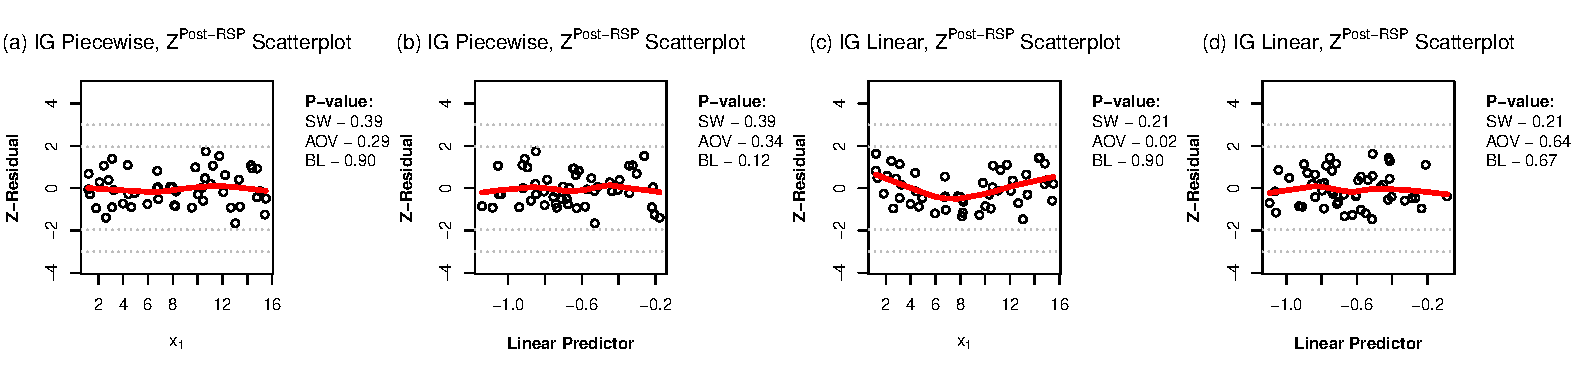
\includegraphics[width=\textwidth, height=0.25\textwidth]{plot/piecewise_ig_fig_n50.pdf}
\caption{Scatterplots of posterior RSP Z-residuals for the continuous IG simulation with sample size $n=50$. Panels (a) and (b) show the correctly specified piecewise IG model, while Panels (c) and (d) show the misspecified linear IG model. }
\label{ig_piecewise_zresid}
\end{figure}


To demonstrate how Z-residuals can detect misspecified functional forms in
this continuous setting, we show posterior RSP Z-residuals from a
representative dataset with $n=50$ in Figure~\ref{ig_piecewise_zresid}. For
the correctly specified piecewise IG model, the residuals are randomly
scattered around zero against both $X_1$ and the fitted linear predictor,
with no discernible trend (Figures~\ref{ig_piecewise_zresid}(a) and (b)).
In contrast, under the misspecified linear IG model, the residual plot
against $X_1$ displays a clear nonlinear pattern, reflecting the true  piecewise quadratic covariate effect
(Figure~\ref{ig_piecewise_zresid}(c)). Notably, no such pattern is visible
in the plot against the fitted linear predictor
(Figure~\ref{ig_piecewise_zresid}(d)): the fitted predictor reduces all
covariates to a single variable, in which the misspecified
linear approximation to the effect of $X_1$ is blended with the remaining
covariate effects, thereby masking the residual curvature associated with
$X_1$. These results illustrate that covariate-specific Z-residual plots
are essential for detecting subtle functional-form misspecifications.

\begin{figure}[ht]
\centering
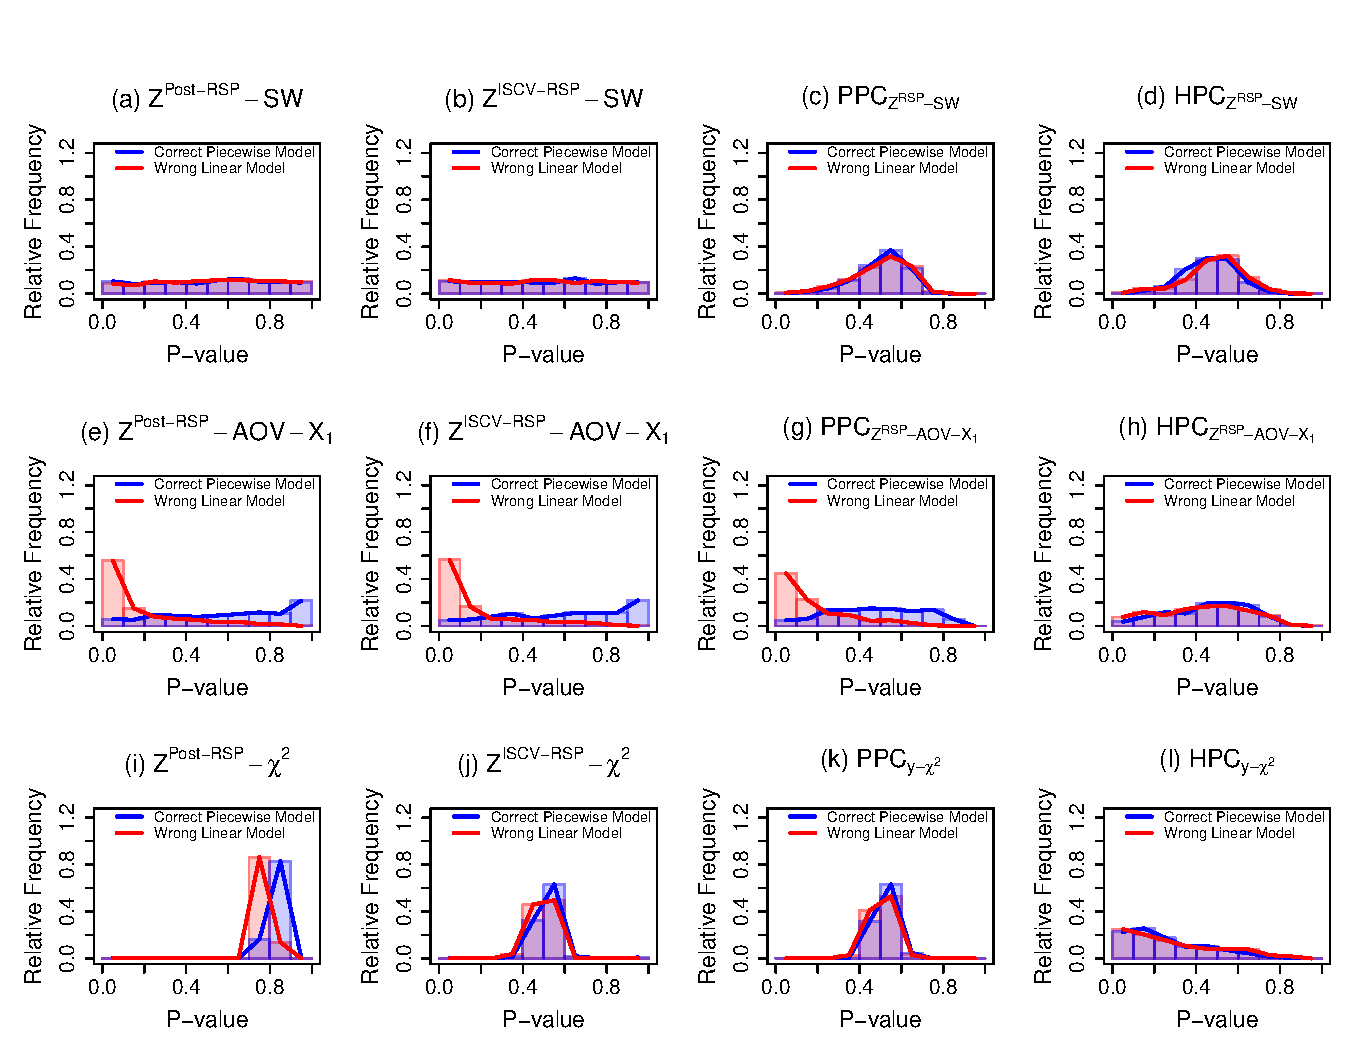
\includegraphics[width=1\textwidth, height=0.7\textwidth]{plot/piecewise_combined_histograms_n50.pdf}
\caption{Empirical $p$-value distributions for various diagnostic methods in the IG simulation with $n=50$. The blue histograms represent the distributions under the correctly specified piecewise IG model, and the red histograms show the distributions under the misspecified linear IG model. The HPC tests use a splitting ratio of $4:1$ for training and testing.}
\label{fig_histogram_ig_n50}
\end{figure}

We then examine the empirical distributions of diagnostic $p$-values based on 500 replications with $n=50$ (Figure~\ref{fig_histogram_ig_n50}). Under the correct piecewise model, the $p$-values of the SW and AOV tests based on posterior and ISCV RSP Z-residuals (panels (a), (b), (e), and (f)) are spread roughly uniformly over the unit interval, indicating good calibration. The AOV tests against $X_1$ (panels (e) and (f)) show the sharpest contrast between models: their $p$-values concentrate strongly near zero under the wrong linear model, as expected, since the misspecification occurs at the functional form of $X_1$, which the AOV diagnostic directly targets. The SW $p$-values (panels (a) and (b)) remain nearly uniform under both models, because the wrong model does not substantially distort the marginal normality of the residuals. The Z-residual $\chi^2$ tests are poorly calibrated even under the correct model, peaking around 0.8 (posterior, panel (i)) or 0.5 (ISCV, panel (j)) under both models, implying deflated Type-I error rates and little sensitivity to the misspecification. The PPC and HPC diagnostics show similar pathologies: panels (c), (d), and (k) are mound-shaped around 0.5 under both models, while HPC$_{y\text{-}\chi^2}$ (panel (l)) is skewed toward small $p$-values under both. Only PPC with the Z-AOV statistic (panel (g)) shifts noticeably toward zero under the wrong model, though less sharply than panels (e) and (f); the corresponding HPC (panel (h)) yields nearly overlapping distributions. In summary, the covariate-specific AOV tests based on posterior and ISCV RSP Z-residuals give the clearest and best-calibrated signal: near-uniform $p$-values under the correct model and strong concentration near zero under the wrong one.

\begin{figure}[ht]
\centering
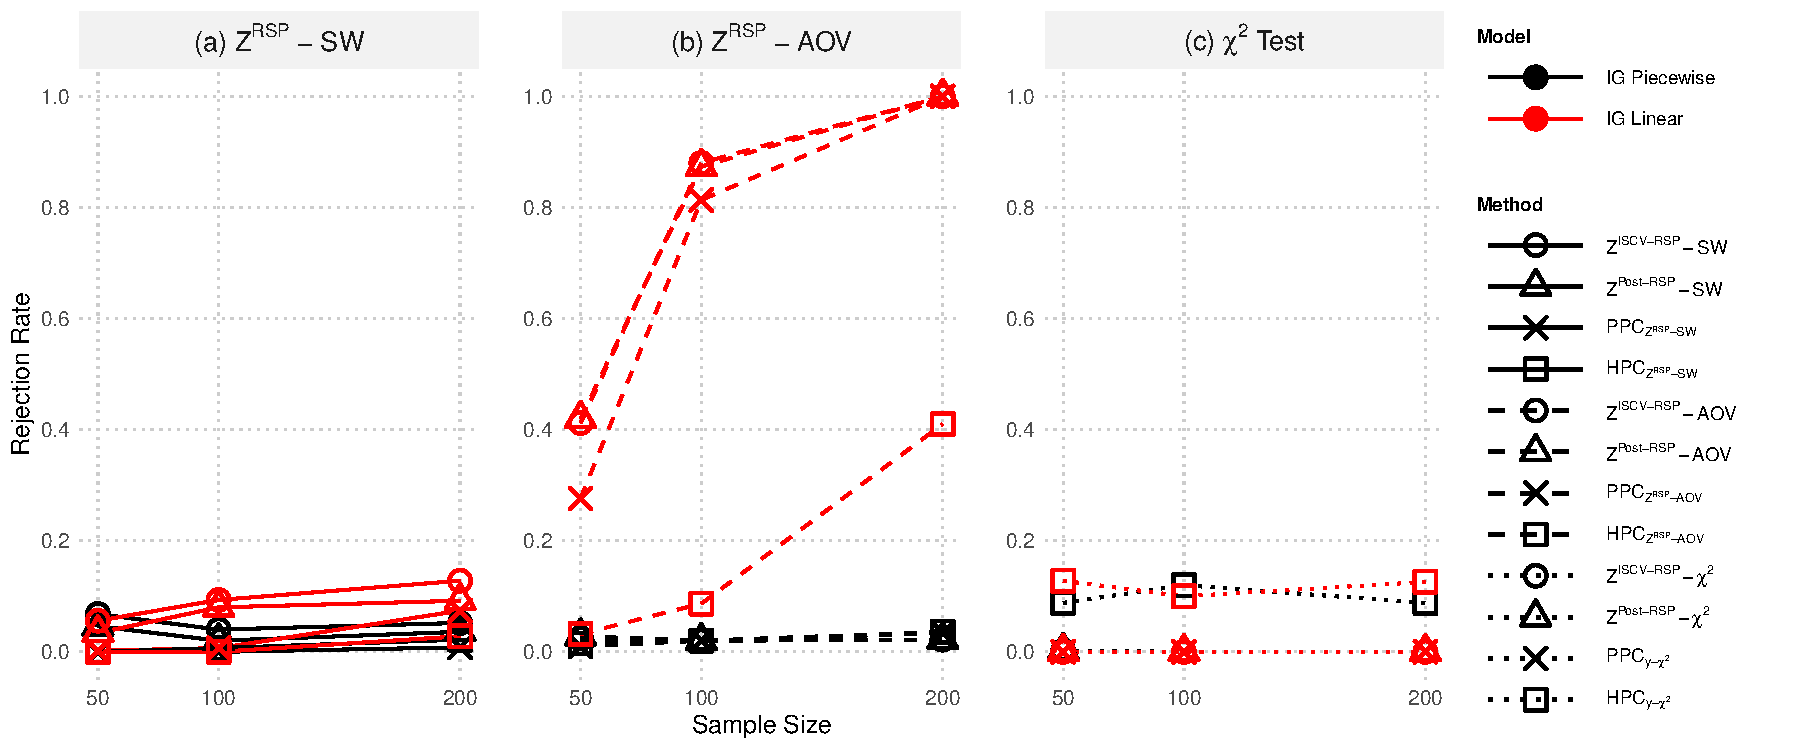
\includegraphics[width=\textwidth, height=0.4\textwidth]{plot/piecewise_rejection_rate_plot.pdf}
\caption{Empirical model rejection rates for various diagnostic methods under different sample sizes $(n=50,100,200)$ in the continuous IG simulation, with a nominal significance level of 0.05. The rejection rates under the correctly specified piecewise IG model are shown in black, and the rates under the misspecified linear IG model are shown in red. The HPC tests use a splitting ratio of $4:1$ for training and testing.}
\label{fig_rejection_rate_ig}
\end{figure}

Figure~\ref{fig_rejection_rate_ig} compares the empirical rejection rates across sample sizes $n=50,100,200$, based on 500 replications and a nominal significance level of 0.05. Numerical rejection rates are reported in Supplementary Table~\ref{S-tab:supp_ig_rejection_rates}. Under the correctly specified piecewise model, the posterior and ISCV RSP Z-residual tests maintain rejection rates close to the nominal level for the SW and AOV diagnostics (panels (a) and (b)), indicating good calibration and valid Type-I error control. Under the misspecified linear model, the SW tests (panel (a)) have little power, with rejection rates below 0.13 even at $n=200$, confirming that an overall normality check is insensitive to this localized nonlinear mean misspecification. The $\chi^2$-based tests (panel (c)) fail on calibration itself: the rejection rates of the Z-residual and PPC $\chi^2$ tests are far below the nominal level under both models (at most 0.002), while the rejection rate of HPC$_{y\text{-}\chi^2}$ is 0.09--0.13 under both, so the nominal cutoff is invalid in either direction and the two models are barely separated. 

In contrast, the Z-residual AOV tests against $X_1$ (panel (b)) combine calibration with power: rejection rates stay near-nominal under the correct model and rise sharply with sample size under the wrong one. In addition, the Z-residual AOV tests have higher rejection rates than the corresponding PPC test at $n=50$ (0.42 versus 0.28) and $n=100$ (0.88 versus 0.81), and all three reach complete rejection at $n=200$. The HPC AOV test is markedly less powerful, with a rejection rate of only 0.41 at $n=200$. 

\subsection{Detecting Nonlinear Covariate Effects in HNB Models}\label{sec:sim-nl}


In this section, we conducted a second simulation study focusing on a hurdle negative binomial (HNB) model. To evaluate the detection of nonlinear mean misspecification in count data, we generated 500 datasets for each sample size $n\in\{50,100,200\}$. Each dataset included covariates $X_1^{(i)} \sim \mathrm{Unif}(0,15)$, binary $X_2^{(i)} \sim \mathrm{Binom}(1,0.5)$, and five standard normal predictors $\bm{Z}^{(i)} = (Z_1^{(i)},\dots,Z_5^{(i)})^\top$ to increase dimensionality. The responses were simulated from an HNB distribution where the count mean $\mu_i$ and the zero-probability $\hu$ were specified directly using the true coefficients: $\log(\mu_i) = -1 + 6\log(X_1^{(i)}) + X_2^{(i)}$ and $\mathrm{logit}(\hu) = -1 - X_1^{(i)} - 5X_2^{(i)}$. This parameterization yielded an overall zero proportion of $\pi^0 \approx 30\%$. For each dataset, we fitted two Bayesian HNB models using \texttt{brms}: a correctly specified \textbf{Logarithmic} model with $\log(X_1^{(i)})$ in the count component, and a misspecified \textbf{Linear} model that incorrectly replaced this term with a linear term of $X_1^{(i)}$. Both models retained the correct zero-model structure and used all other covariates.

To demonstrate the covariate-specific diagnostic, we show posterior RSP Z-residuals from a representative dataset in Figure~\ref{fig_scatter_boxplot_sim2}. Under the specified logarithmic HNB model, the residuals show no discernible trend against $X_1$, and the grouped boxplots are approximately homogeneous, supported by a non-significant AOV test with $p$-value $>0.05$ (Figures~\ref{fig_scatter_boxplot_sim2}(a) and (b)). In contrast, the misspecified linear HNB model produces a clear residual pattern and pronounced grouped mean differences across $X_1$, detected by the AOV test with $p$-value $<0.01$ (Figures~\ref{fig_scatter_boxplot_sim2}(c) and (d)). These results show that Z-residual plots and covariate-specific grouped tests can identify misspecified functional forms in discrete HNB models.
\begin{figure}[ht]
\centering
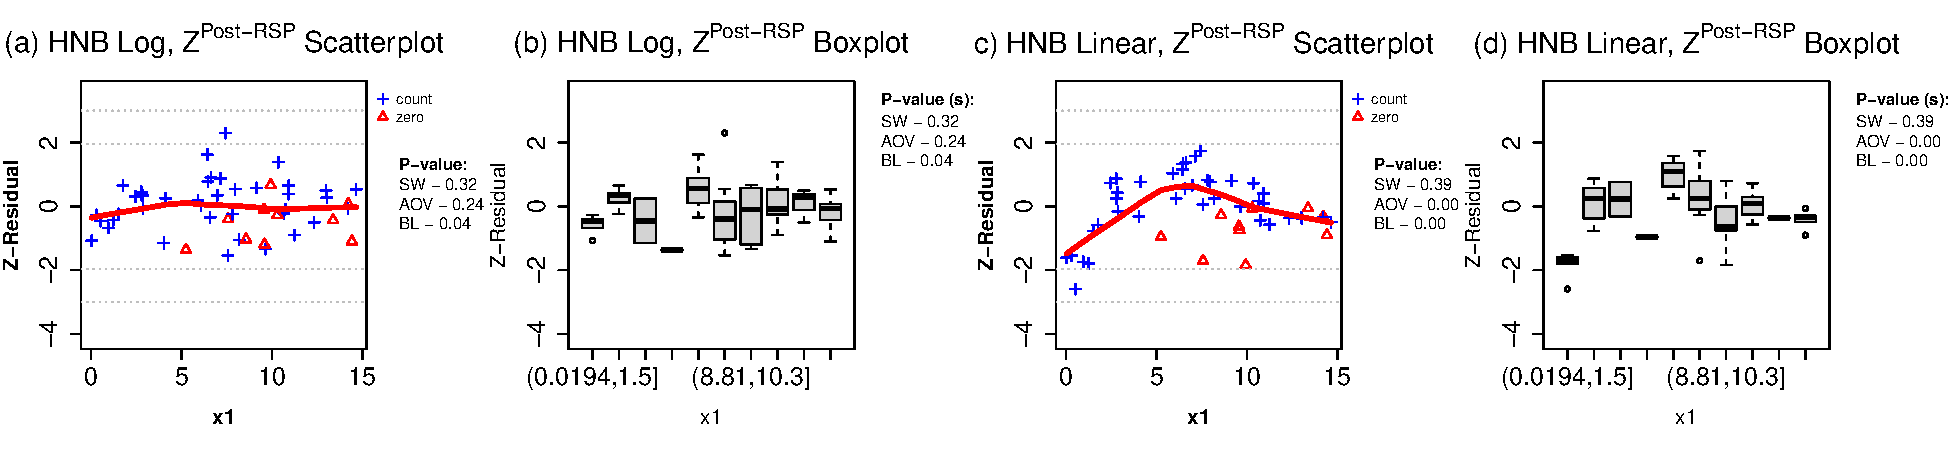
\includegraphics[width=\textwidth, height=0.25\textwidth]{plot/sim2_HNB_scatter_box_plot.pdf}
\caption{Visual diagnostics of posterior RSP Z-residuals for HNB models with logarithmic (true) and linear (wrong) covariate effects, based on a representative dataset with sample size $n=50$. Panels (a) and (c) display scatterplots of the posterior RSP Z-residuals against covariate $X_1$, with positive count observations shown as blue crosses and zero observations shown as red triangles. Panels (b) and (d) present the boxplots of Z-residuals grouped  by $X_1$.}
\label{fig_scatter_boxplot_sim2}
\end{figure}

We then examine the empirical distributions of diagnostic $p$-values using replicated datasets, as displayed in Figure~\ref{fig_histogram_sim2}. The histograms are based on 500 replications with $n=50$ and an overall zero proportion of $\mhu\approx30\%$. Consistent with the continuous IG simulation, the covariate-specific AOV diagnostics provide the clearest signal. The SW tests on posterior and ISCV RSP Z-residuals are approximately calibrated under the true logarithmic HNB model, but their separation between the true and wrong models is weaker than that of the AOV tests (Figures~\ref{fig_histogram_sim2}(a) and (b)). In contrast, the AOV tests against $X_1$ based on posterior and ISCV Z-residuals are well calibrated under the true model and highly powerful under the misspecified linear model, with $p$-values heavily concentrated near zero (Figures~\ref{fig_histogram_sim2}(e) and (f)).

The corresponding PPC and HPC methods are more poorly calibrated and less powerful. The PPC and HPC checks based on SW have $p$-values concentrated around 0.5 and provide little separation (Figures~\ref{fig_histogram_sim2}(c) and (d)). The PPC AOV check has high power under the wrong model, but its null $p$-values are again biased toward 0.5 rather than uniformly distributed (Figure~\ref{fig_histogram_sim2}(g)); the HPC AOV check shows only weak separation (Figure~\ref{fig_histogram_sim2}(h)). The $\chi^2$-based checks are less targeted to this functional-form error and do not distinguish the two models as clearly as the Z-residual AOV diagnostics (Figures~\ref{fig_histogram_sim2}(i)--(l)). Overall, the Z-residual-based AOV tests are the most powerful and well-calibrated in this discrete setting.


\begin{figure}[ht]
\centering
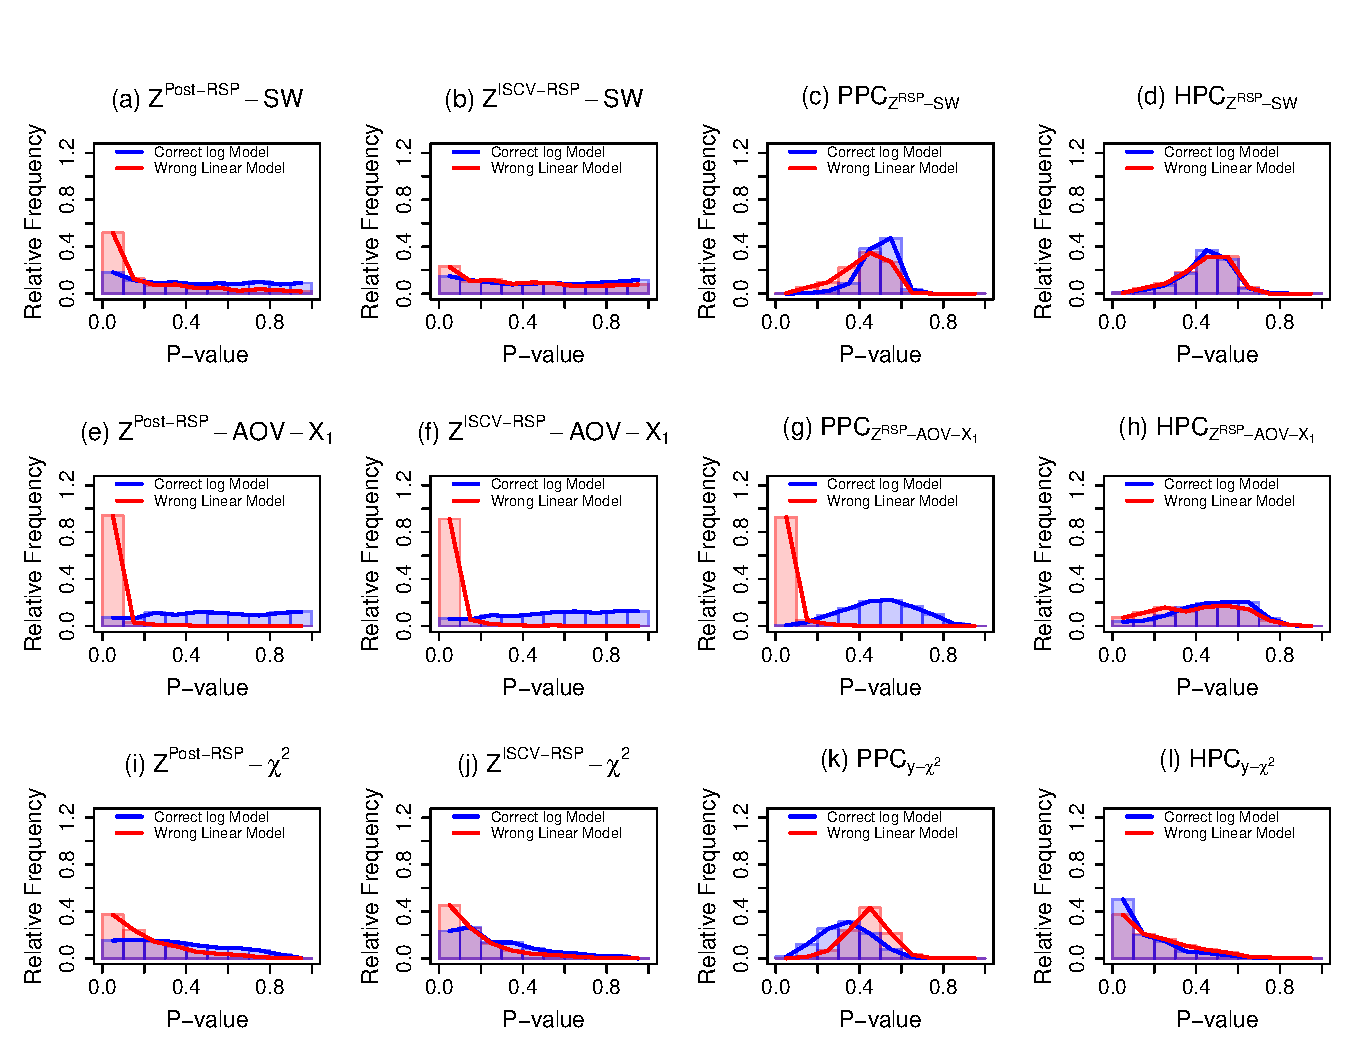
\includegraphics[width=1\textwidth, height=0.8\textwidth]{plot/sim2_hnb_combined_histograms_n50.pdf}
\caption{Empirical $p$-value distributions for various diagnostic methods in the nonlinear HNB simulation with sample size $n=50$ and overall zero proportion $\mhu\approx 30\%$. The blue histograms represent the distributions under the correctly specified logarithmic HNB model, and the red histograms represent the distributions under the misspecified linear HNB model. The HPC tests use a splitting ratio of $4:1$ for training and testing.}
\label{fig_histogram_sim2}
\end{figure}


Finally, Figure~\ref{fig_rejection_rate_sim2} compares model rejection rates across $n=50,100,200$. The corresponding numerical rejection rates are reported in Supplementary Table~\ref{S-tab:supp_hnb_nonlinear_rejection_rates}. The SW tests based on posterior and ISCV RSP Z-residuals maintain Type I error rates near 0.05 and show increasing power under the misspecified linear model, whereas the corresponding PPC and HPC checks have rejection rates close to zero or provide much weaker separation (Figure~\ref{fig_rejection_rate_sim2}(a)). The $\chi^2$-based checks are also less informative: the Z-residual $\chi^2$ tests show some power but remain well below the AOV tests, while the PPC and HPC $\chi^2$ checks are generally weak or unstable (Figure~\ref{fig_rejection_rate_sim2}(c)). The AOV-based diagnostics provide the clearest results (Figure~\ref{fig_rejection_rate_sim2}(b)): the posterior and ISCV Z-residual AOV tests maintain low rejection rates under the true model and achieve high power under the misspecified linear model, reaching nearly complete rejection for $n\ge100$. The PPC AOV check also has high power but is lower at $n=50$, whereas the HPC AOV check is less powerful at small sample sizes. These rejection-rate results confirm that covariate-specific AOV tests on Z-residuals provide the strongest diagnostic signal for nonlinear functional-form misspecification in this discrete HNB simulation. 
\begin{figure}[htp]
\centering
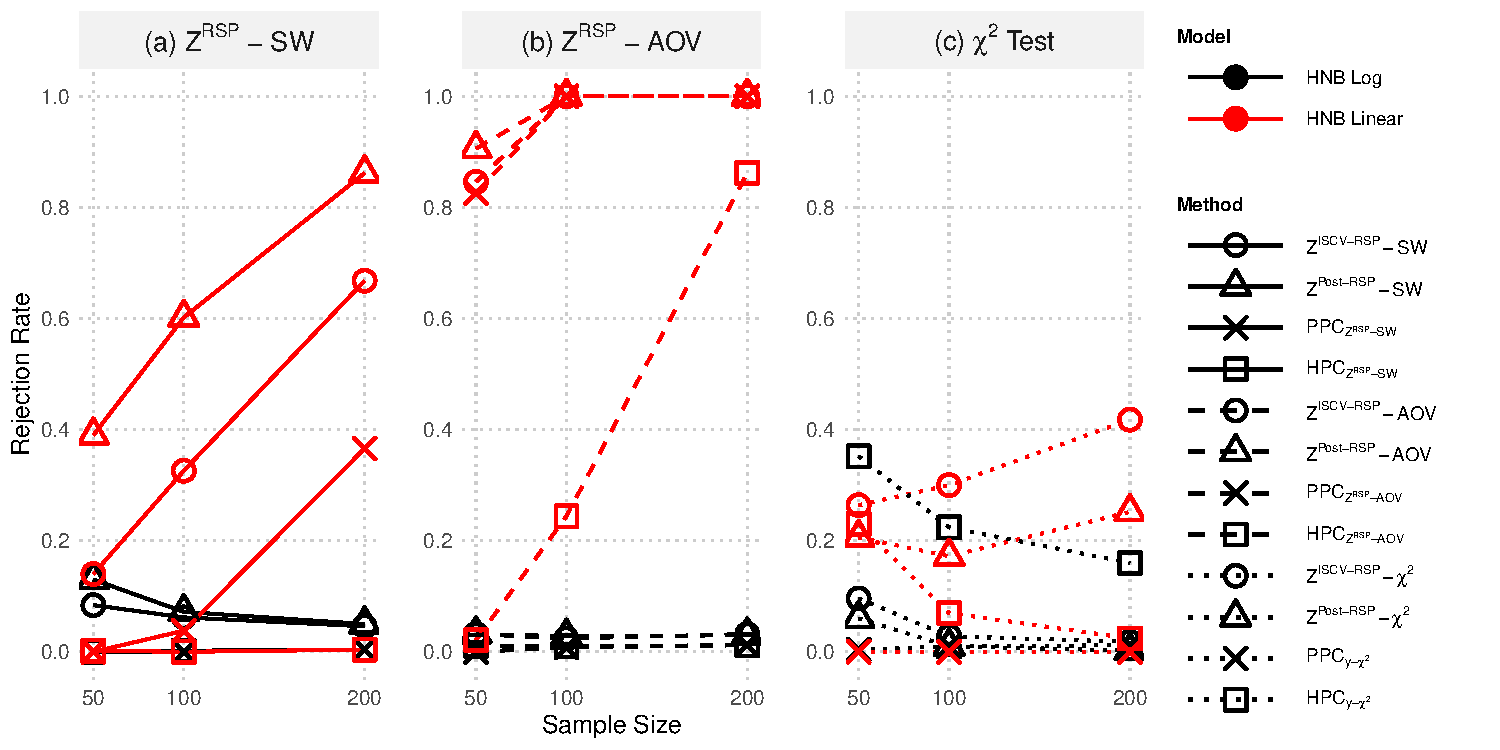
\includegraphics[width=1\textwidth]{plot/sim2_hurdle_nl_rejection_rate_plot.pdf}
\caption{Empirical model rejection rates for various diagnostic methods under different sample sizes ($n=50, 100, 200$), with a nominal significance level of 0.05. The rejection rates under the true logarithmic HNB model (Type I error) are shown in black, and the rates under the wrong linear HNB model (power) are shown in red. The HPC tests use a splitting ratio of $4:1$ for training and testing.
}
\label{fig_rejection_rate_sim2}
\end{figure}

In summary, the simulation results show that the AOV tests on Z-residuals give significantly higher power than overall goodness-of-fit tests such as SW and $\chi^2$ tests in detecting mis-specified covariate functional forms. The PPC method with AOV test can also achieve high power. However, visual diagnostics of Z-residuals, such as the scatterplots and boxplots in Figure~\ref{fig_scatter_boxplot_sim2}, can inform the selection of an appropriate test for a PPC. 

\textred{A supplementary sensitivity analysis (Section~\ref{S-sec:sens_family_function}) fits NB-log and NB-linear models to the same HNB-generated data to examine how response-family misspecification interacts with the residual-versus-$X_1$ diagnostics. While a functional-form deficiency remains detectable under the misspecified NB family, the results highlight the critical power of a joint analysis. Severe misspecification in one model component can cascade into diagnostics targeting another---for instance, an incorrect response family can distort the implied mean structure---meaning no single test provides a complete picture. By evaluating numerical and graphical residual diagnostics jointly, practitioners gain significantly more leverage to disentangle these interacting model deficiencies, even though isolating the exact source of misfit remains challenging; see Section~\ref{S-sec:sens_family_function} for a detailed discussion.}

\section{Applications to a Zero-inflated Dataset}\label{real_data}

This section applies Z-residual diagnostics in parallel with PPC methods to a real dataset. We analyze the dolphin-sighting data from Chapter~7 of  \citet{TheWorldofZeroInflatedModels}, which draws on publicly available sources including \citet{JacksonRickettsJustine2020HmoI}. The dataset contains $n=936$ observations. The response is the count of dolphin sightings;  covariates include water depth (\texttt{depth}), water temperature (\texttt{temp}), distance to the river mouth (\texttt{dr}, indexing the estuarine–coastal gradient), \texttt{salinity}, \texttt{turbidity}, survey \texttt{year} and a location identifier. Because zeros are prevalent (about $75\%$), we fit four regression families: hurdle Poisson, hurdle negative binomial (HNB), Poisson, and negative binomial (NB). We then assess overall goodness-of-fit and the functional forms of covariate effects using posterior Z–residual diagnostics alongside PPC methods.


We first fit each family with \emph{linear} covariate effects and evaluate overall goodness-of-fit using \textbf{posterior RSP Z–residuals}. Figure~\ref{realdata_qqplot} shows QQ–plots of posterior RSP Z–residuals. The QQ-plots of the HNB and NB models adhere closely to the diagonal lines, suggesting adequate fit, whereas the QQ-plots of the hurdle Poisson and Poisson models deviate markedly from the diagonal lines, especially in their upper tails. The $Z^{\text{Post-RSP}}\text{-SW}$ $p$-values beside the QQ-plots also confirm numerically these impressions: HNB  and NB models having $p$-values $\geq 0.05$ (no rejection) versus hurdle Poisson and Poisson both having $<0.01$ $p$-values (clear rejection). It is clear that the Poisson family cannot model well the strong overdispersion and the hurdle modification does not improve it.


\begin{figure}[htp]
\centering
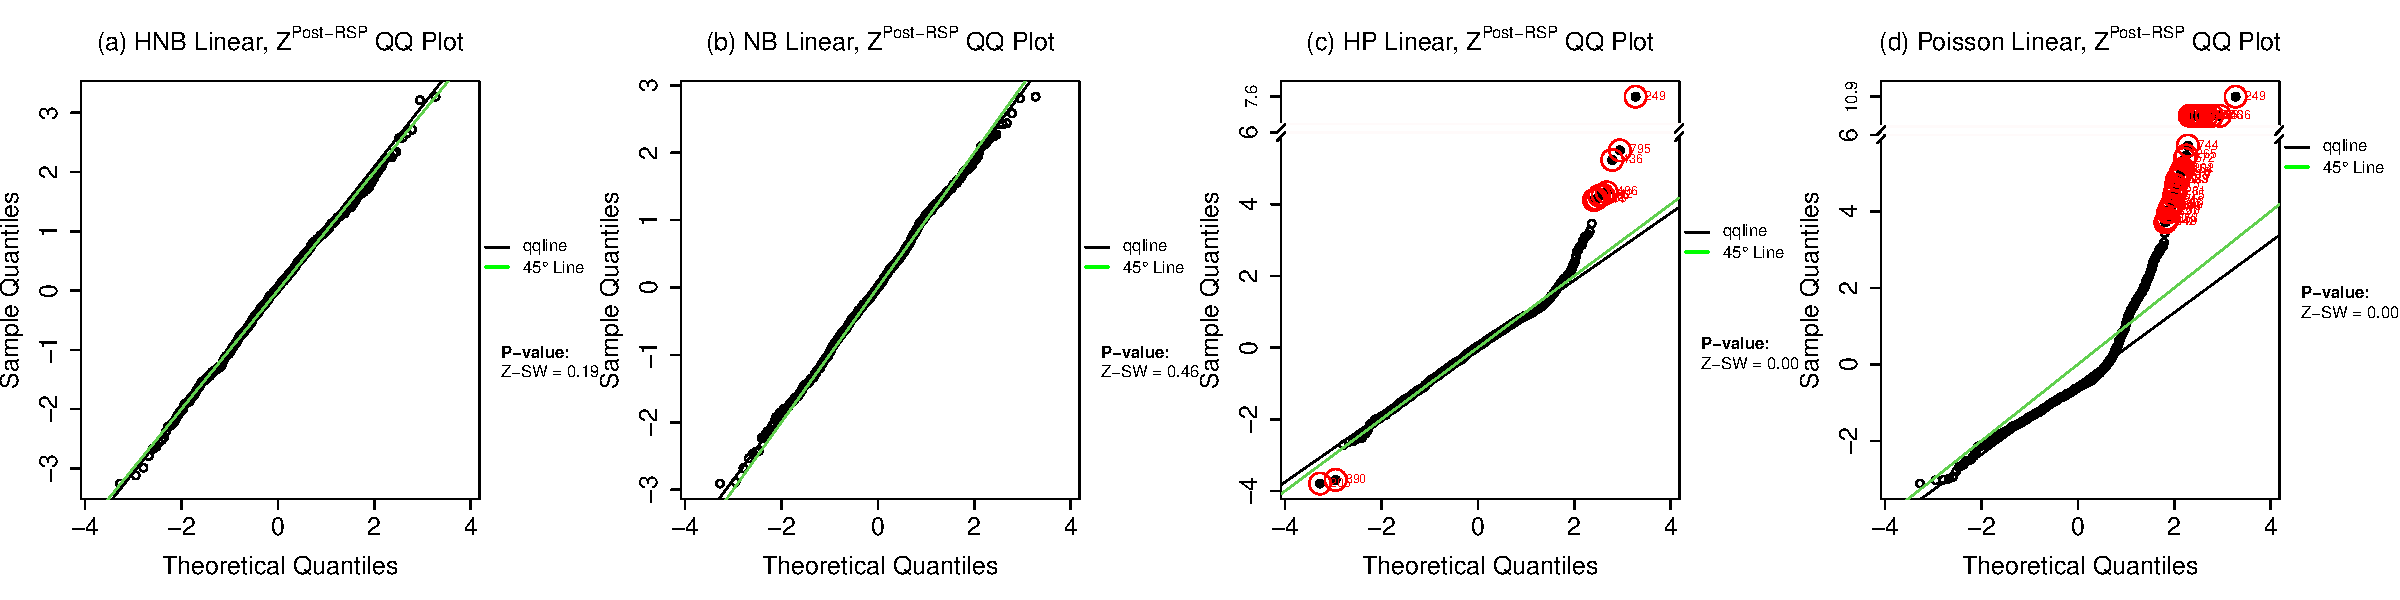
\includegraphics[width=\textwidth, height=0.25\textwidth]{plot/realdata_qqplot.pdf}
\caption{QQ plots of posterior RSP Z-residuals for the (a) HNB, (b) NB, (c) hurdle Poisson, and (d) Poisson models, each fitted in linear form to the dolphin-sighting dataset.}
\label{realdata_qqplot}
\end{figure}


Given the overall adequacy of HNB and NB, we next examine covariate functional forms using posterior Z-residual diagnostics, focusing on the AOV $F$ test ($Z^{\text{Post-RSP}}\text{-AOV}$). As shown in Figure~\ref{fig-realdata_linear_plot} for the linear HNB model, plotting Z-residuals against \texttt{depth} reveals a clear U-shape (Figure~\ref{fig-realdata_linear_plot}a) and heterogeneous boxplots across \texttt{depth} groups (Figure~\ref{fig-realdata_linear_plot}b), indicating a potential misspecification of the functional form for \texttt{depth}. The $Z^{\text{Post-RSP}}\text{-AOV}$ test yields a $p$-value $<0.01$, strongly rejecting the hypothesis of equal Z-residual means across the \texttt{depth} groups. To examine robustness with respect to the auxiliary randomization $U$ (for discrete outcomes), we drew 500 sets of $\bU$, computed the $Z^{\text{Post-RSP}}\text{-SW}$ and $Z^{\text{Post-RSP}}\text{-AOV}$ $p$-values for each set, and summarized the replicated $p$-values using the conservative upper-bound for the median (Sec.~\ref{ZRESID}; Eq.~\eqref{eqn:uppvalue-median}). Figures~\ref{fig-realdata_linear_plot}(c) and (d) display the replicated $p$-value histograms, with red lines marking the upper-bounds. For $Z^{\text{Post-RSP}}\text{-AOV}$ (d), most $p$-values fall below $0.05$, with a median upper-bound of $0.012$, revealing a significant nonlinear effect of \texttt{depth}. The $p$-values for $\text{PPC}_{Z^{\text{RSP}}\text{-SW}}$ and $\text{PPC}_{Z^{\text{RSP}}\text{-AOV}}$ in Table~\ref{realdata_pvalue} support this finding. In contrast, the $Z^{\text{Post-RSP}}\text{-SW}$ test (c) yields $p$-values mostly above $0.05$, with a median upper-bound of $0.790$ (Table~\ref{realdata_pvalue}). This finding supports the conclusion from Section~\ref{sec:sim-nl}: overall goodness-of-fit tests such as SW can lack power for detecting nonlinearity.
\begin{figure}[htp]
\centering
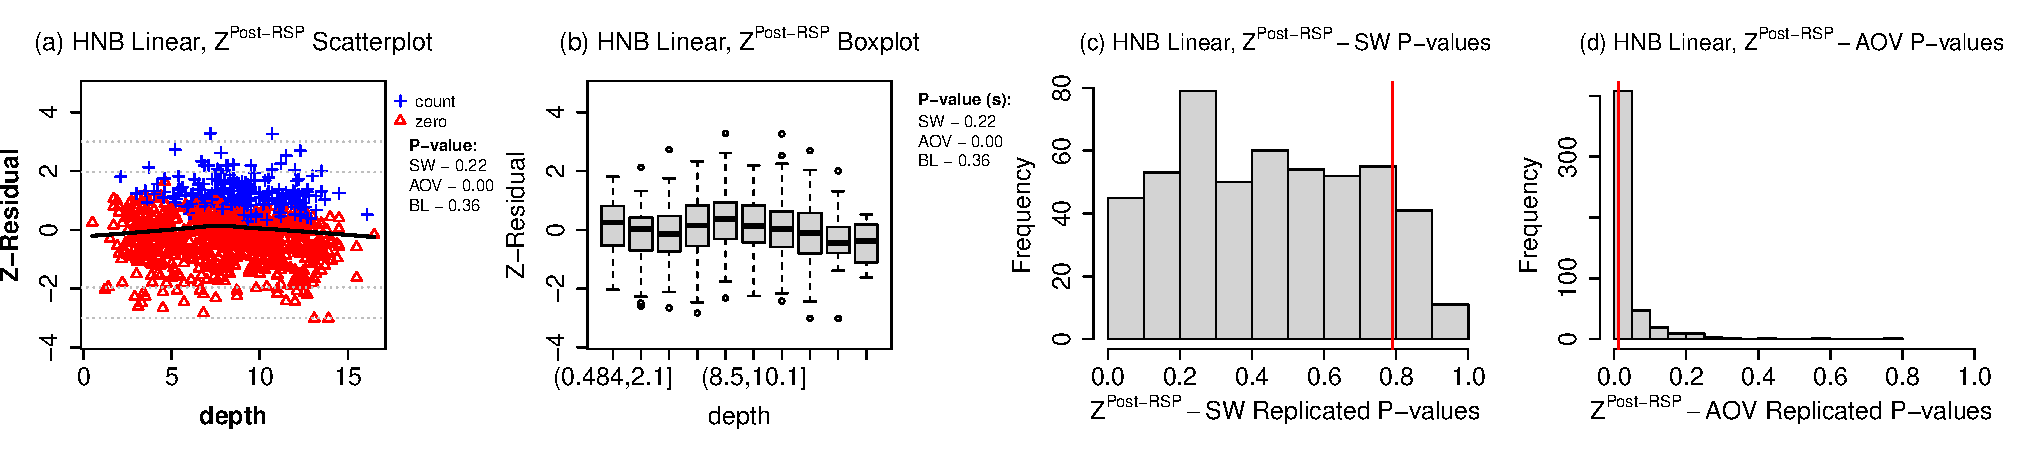
\includegraphics[width=\textwidth, height=0.25\textwidth]{plot/realdata_plot_linear.pdf}
\caption{Posterior RSP Z-residual diagnostics for nonlinearity in the linear HNB model for the dolphin-sighting data. (a):~scatterplot and (b):~grouped boxplots of Z-residuals versus \texttt{depth}, with non-zeros as blue crosses and zeros as red triangles.  (c, d):~histograms of 500 replicated $p$-values for the $Z^{\text{Post-RSP}}\text{-SW}$ and $Z^{\text{Post-RSP}}\text{-AOV}$ tests, respectively; red lines mark the upper-bound for the median.}
\label{fig-realdata_linear_plot}
\end{figure}

After rejecting a linear term for \texttt{depth}, we specified a piecewise quadratic effect to better capture the nonlinearity. This choice was informed by the scatterplot in Figure~\ref{fig-realdata_linear_plot}(a), which shows a clear turning point at \texttt{depth} = 7.95. We created two corresponding variables: $\texttt{below7.95} = \{(\texttt{depth}-7.95)^2\}\,\mathbf{1}(\texttt{depth}<7.95)$ and $\texttt{above7.95} = \{(\texttt{depth}-7.95)^2\}\,\mathbf{1}(\texttt{depth}\ge 7.95)$. After refitting the HNB model with these two variables, the diagnostic results in Figure~\ref{fig-realdata_nonlinear_plot} confirmed a substantially improved fit. The scatterplot (a) and boxplots (b) now display randomly scattered, homogeneous Z-residuals with no visible patterns, indicating that the nonlinear effect of \texttt{depth} has been successfully modeled. The large $Z^{\text{Post-RSP}}\text{-AOV}$ $p$-value of $0.88$ numerically supports this conclusion. Furthermore, the histograms (c, d) show that the replicated $p$-values for both the $Z^{\text{Post-RSP}}\text{-SW}$ and $Z^{\text{Post-RSP}}\text{-AOV}$ tests are now mostly above $0.05$. As summarized in the Nonlinear panel of Table~\ref{realdata_pvalue}, the Z-residuals for both the nonlinear HNB and NB models yield large median upper-bound $p$-values; for instance, the Z-SW and Z-AOV tests applied to the HNB model resulted in $p$-values of $0.969$ and $1.000$, respectively. The PPC tests using Z-SW and Z-AOV also yield large $p$-values for these two models. Finally, a comparison of the models using the LOO expected log point-wise predictive density (elpd), shown in the  \texttt{elpd} column of Table~\ref{realdata_pvalue}, confirms that the HNB model with a nonlinear \texttt{depth} effect significantly improves the fit over the linear version and also outperforms the NB models.


\begin{figure}[htp]
\centering
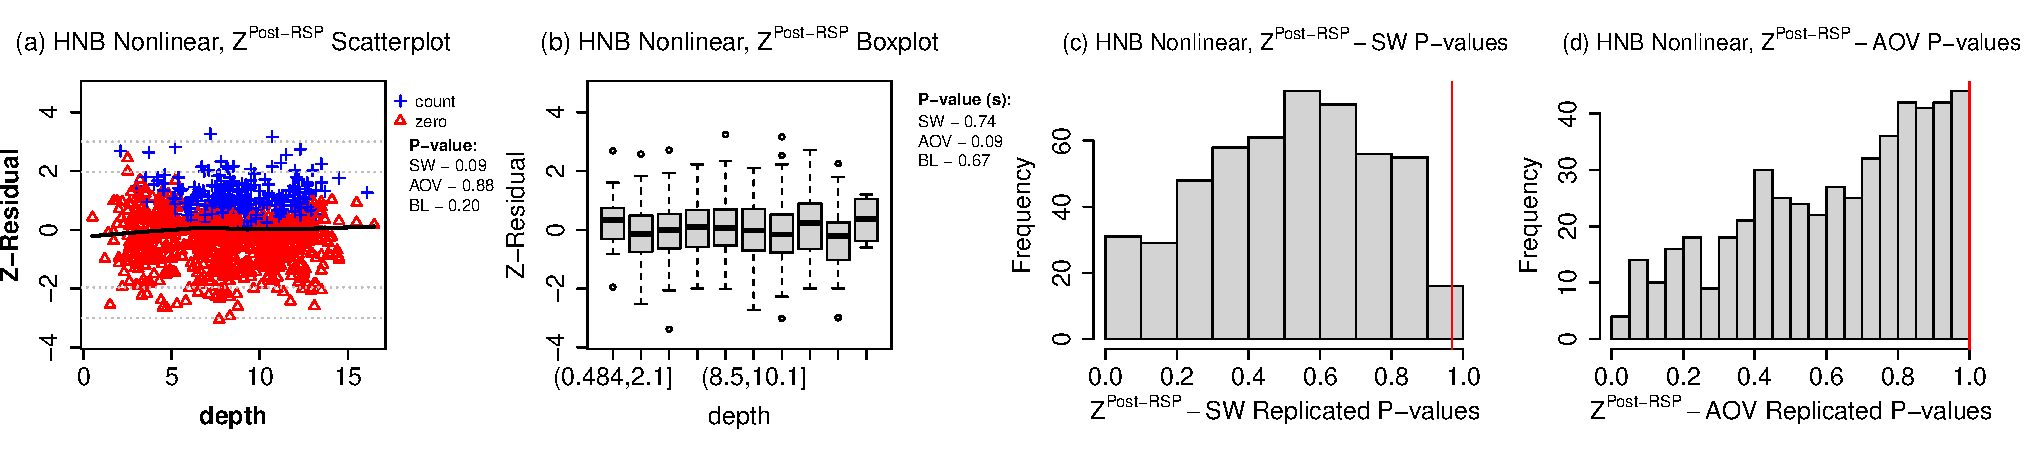
\includegraphics[width=\textwidth, height=0.25\textwidth]{plot/realdata_plot_nonlinear.pdf}
\caption{Diagnostics based on posterior RSP Z-residuals for the HNB nonlinear model fitted to the dolphin-sighting data. Panels (a) and (b) show a scatterplot and a boxplot of the posterior RSP Z-residuals against \texttt{depth}, distinguishing counts observations (blue crosses) from zeros observations (red triangles). Panels (c) and (d) display histograms of 500 replicated $p$-values for $Z^{\text{Post-RSP}}\text{-SW}$ and $Z^{\text{Post-RSP}}\text{-AOV}$ $p$-values.}
\label{fig-realdata_nonlinear_plot}
\end{figure}



\textred{The $\text{PPC}_{y-\chi^2}$ results (Table~\ref{realdata_pvalue}, PPC columns) differ from the other diagnostic results in this example.} This test rejects both the linear HNB ($p=0.017$) and the nonlinear HNB ($p=0.024$) while accepting the NB variants. Because both Z-residual diagnostics and \PPC\ Z-residual tests indicate adequate fit for the nonlinear HNB and NB models, we adjudicate using out-of-sample performance via LOO expected log predictive density (elpd). The LOO comparison across all six candidates ranks the nonlinear HNB first ($\Delta_{\text{elpd}}=0$), followed by linear HNB ($-20.4$, se $=6.8$), nonlinear NB ($-34.1$, se $=9.9$), linear NB ($-43.0$, se $=10.0$), and then Poisson-based models. Thus, while both HNB and NB families can fit adequately once the nonlinearity is addressed, \textred{the nonlinear HNB has the highest \texttt{elpd} among the fitted candidate models.} 
\begin{table}[htbp]
\centering
\caption{\textred{Diagnostic $p$-values and LOO comparisons for the dolphin-sighting data. Rows are grouped into four linear models (HNB, NB, hurdle Poisson, Poisson) and two nonlinear models (HNB, NB). For posterior and ISCV Z-residual tests, we report median upper-bound $p$-values~(eq.~\eqref{eqn:uppvalue-median}); all Z-AOV tests are conducted against \texttt{depth}. The last three columns report $\Delta_{\text{elpd}}$ relative to the nonlinear HNB model, its standard error, and $\Pr(\Delta_{\text{elpd}}\ge 0)$.The HPC tests use a splitting ratio of $4:1$ for training and testing.}}
\label{realdata_pvalue}

\setlength{\tabcolsep}{6pt}
\resizebox{\textwidth}{!}{
\begin{tabular}{lrrrrrrrrrrrrrrr} 
\toprule
& \multicolumn{3}{c}{\textbf{Post. Z-Residual Tests}}
& \multicolumn{3}{c}{\textbf{ISCV Z-Residual Tests}}
& \multicolumn{3}{c}{\textbf{PPC Tests}}
& \multicolumn{3}{c}{\textbf{HPC Tests}}
& \multicolumn{3}{c}{\textbf{LOO Comparison}} \\
\cmidrule(lr){2-4} 
\cmidrule(lr){5-7}
\cmidrule(lr){8-10}
\cmidrule(lr){11-13} 
\cmidrule(lr){14-16}
Family 
& Z-SW & Z-AOV & Z-$\chi^2$ 
& Z-SW & Z-AOV & Z-$\chi^2$ 
& Z-SW & Z-AOV & $y-\chi^2$ 
& Z-SW & Z-AOV & $y-\chi^2$ 
& $\Delta_{\text{elpd}}$ & SE & $\Pr(\Delta_{\text{elpd}} \ge 0)$\\
\midrule
\multicolumn{16}{l}{\textit{Linear models}} \\
HNB 
& 0.790 & 0.012 & 0.823 
& 0.395 & 0.013 & 0.316 
& 0.674 & 0.035 & 0.017 
& 0.609 & 0.369 & 0.250 
& -19.9 & 6.8 & 0.002 \\

NB  
& 0.299 & 0.010 & 0.948 
& 0.880 & 0.009 & 0.520 
& 0.392 & 0.026 & 0.538 
& 0.530 & 0.403 & 0.691  
& -42.5 & 9.9 & $<0.001$ \\

HP  
& $<0.01$ & 0.020 & $<0.01$ 
& $<0.01$ & 0.022 & $<0.01$ 
& $<0.01$ & 0.041 & $<0.01$ 
& $<0.01$ & 0.324 & $<0.01$  
& -118.6 & 34.4 & $<0.001$ \\

Poisson 
& $<0.01$ & 0.012 & $<0.01$ 
& $<0.01$ & 0.015 & $<0.01$ 
& $<0.01$ & 0.013 & $<0.01$ 
& $<0.01$ & 0.340 & $<0.01$ 
& -803.3 & 101.1 & $<0.001$ \\

\midrule
\multicolumn{16}{l}{\textit{Nonlinear models}} \\
HNB 
& 1.000 & 1.000 & 0.732 
& 0.534 & 1.000 & 0.262  
& 0.616 & 0.575 & 0.024 
& 0.593 & 0.518 & 0.348 
& 0.0 & 0.0 & \text{Ref.} \\

NB  
& 0.337 & 0.760 & 0.905 
& 0.031 & 0.650 & 0.372  
& 0.149 & 0.372 & 0.169 
& 0.478 & 0.538 & 0.755  
& -34.0 & 9.9 & $<0.001$ \\
\bottomrule
\end{tabular}
}
\end{table}

Two factors plausibly explain the $\text{PPC}_{y-\chi^2}$ rejections. First, posterior predictive $p$-values (PPP) are not uniform under the null because the data are used twice. For some discrepancy measures and replication schemes, they can even be anti-conservative (under-dispersed), inflating the Type I error rate rather than merely reducing power, as reported by \citep[e.g.,][]{BerkhofJohannes2000PpcP,RubinDelanchyPatrick2014Pppa}. Second, the response variable is extremely sparse ($\sim\!75\%$ zeros, with most positive counts $\leq 5$), yielding many cases with very small model-expected counts. The $\text{PPC}_{y-\chi^2}$ checks are then dominated by these cases, which magnify innocuous random fluctuations and trigger spurious rejections; similar inflation has been observed in other incomplete or sparse-data settings \citep[e.g.,][]{XuDandan2016Anop}. We conducted small-scale simulation studies with datasets generated from HNB models with a large overall proportion of zeros ($\approx 70\%$) and observed that the $\text{PPC}_{y-\chi^2}$ test produced similarly high rejection rates (nearly $100\%$) for these correctly specified HNB models. 

\textred{We further conducted two sensitivity checks for the real-data conclusions. First, refitting the candidate models under baseline, tighter, and more diffuse priors yielded qualitatively unchanged Z-residual, PPC, and HPC conclusions (Section~\ref{S-prior_analysis}, Table~\ref{S-tab:prior_sensitivity_specs}, and Figure~\ref{S-fig_prior_sensitivity}). Second, repeating the depth-based grouped diagnostic with \(k \in \{5,10,15,20\}\) equally spaced intervals showed that the conclusion was not driven by the binning choice: the linear HNB model consistently retained residual mean differences across depth groups, whereas the nonlinear HNB model did not (Section~\ref{S-sec:aov_bin_analysis}, Table~\ref{S-tab:binning_sensitivity_pbound}, and Figure~\ref{S-fig_binning_sensitivity}).}


Full regression coefficients for the nonlinear HNB model are available in Table~\ref{S-tab:reg_coefs}. These results show the effect of \texttt{depth} is primarily on the model's hurdle (zero-inflation) component. The estimated coefficients for the hurdle part are $\hat\beta_{\texttt{hu\_below7.95}} = 0.12$ (CI: [0.08, 0.16]) and $\hat\beta_{\texttt{hu\_above7.95}} = 0.03$ (CI: [0.01, 0.05]). This means the odds of a zero count increase by factors of roughly 1.13 and 1.03 for each unit increase in $(\texttt{depth}-7.95)^2$ below and above the 7.95m threshold, respectively. Conversely, the coefficients for the count component are not significant (their credible intervals include zero), which suggests that expected positive counts don't vary substantially with 	\texttt{depth}. Together, these results quantify the U-shaped relationship seen in diagnostics: the probability of a zero count is minimized around 7.95m and increases away from this point, especially in shallower waters.


\section{\textred{Conclusions and Discussions}}\label{concl}

In this paper, we have introduced a versatile Bayesian residual diagnostic
based on RSPs. Mapping posterior or ISCV RSPs through the standard normal
quantile function yields Z-residuals that support familiar graphical and
quantitative diagnostics. The distinctive feature of our approach is its
\emph{summarize-first, then-test} workflow: rather than testing
conditionally on each parameter draw and then summarizing the resulting
$p$-values, we integrate the RSPs over
the posterior or LOOCV distribution to produce a
\emph{single} set of residuals that are asymptotically distributed as
 $N(0,1)$ under a correctly specified model.

In two simulation studies with misspecified covariate functional forms in
IG and HNB models, the proposed Z-residual-based tests yielded well-calibrated Type-I error
rates and greater power for rejecting misspecified models than traditional
PPC and HPC. The simulations also showed that relying solely on the
marginal residual distribution is often insufficient: omnibus tests such as
the Shapiro--Wilk (SW) and $\chi^2$ tests masked structural flaws that
covariate-specific $Z$--AOV tests readily detected, underscoring the value
of graphical Z-residual summaries as exploratory tools that expose unknown
deficiencies and guide formal testing. Moreover, by averaging over MCMC
draws, Z-residual-based PPC remained stable despite the auxiliary $\bm{U}$
drawn at each iteration, mitigating the double-use-of-data conservatism of
traditional $\chi^2$ PPC. Finally, applying the framework to the
dolphin-sighting dataset exposed a nonlinear depth effect, guiding a
revision to a nonlinear HNB model that passed all diagnostic checks and
improved predictive performance as measured by LOO \texttt{elpd}.

The core strength of the Z-residual framework lies in assessing the approximated predictive distribution (posterior or ISCV) against the actually observed $y_i$. Because this predictive distribution converges to the true data-generating distribution as the sample size increases, our method yields observation-level residuals that are asymptotically normal under the null. However, this strict observation-level focus entails an inherent \textbf{limitation}: the method is largely insensitive to non-observation-level components, such as latent variables, hierarchical effects, and priors. Consequently, the proposed Z-residuals are less effective at detecting misspecification within a model's internal structure.

To address this limitation, a highly promising direction for future work is to extend the RSP framework to the evaluation of internal model components, drawing inspiration from Uniform Parametrization Checks (UPC) \citep{covington2025bayesian}. For a single posterior draw $\btheta^{(t)}$, UPC shares a fundamental mathematical equivalence with RSPs: its observation-level uniform variables are distributionally identical to $1 - \rsp_i(y_i \mid \btheta^{(t)})$. The two frameworks diverge, however, in how they aggregate over the posterior. UPC adopts a ``test-first, then-summarize'' approach, combining MCMC-wise $p$-values via the Cauchy combination rule \citep{liu2020cauchy}---a highly innovative strategy, although its approximation error may not fully vanish asymptotically. Combining UPC's novel perspective on internal random components with the asymptotic stability of our ``summarize-first'' RSP framework offers an interesting avenue for diagnosing latent structures. For this combination to succeed, the primary methodological challenge will be to formally define what constitutes an ``observed'' value for these internal components, so that their corresponding RSPs can be validly constructed and assessed.

Beyond extending the methodology to the assessment of latent variables, several practical enhancements could further strengthen the current Z-residual framework. One immediate challenge arises when applying Z-residuals to \emph{discrete} responses: the auxiliary randomness $\bU$ causes the resulting test $p$-values to vary across random seeds. Because practitioners often require a single representative value, we recommend re-randomizing $\bU$ multiple times and summarizing the replicated $p$-values with an order statistic $p_{(r)}$, such as the median. To this end, we derived a distribution-free, super-uniform upper bound $H_{J,r}\, p_{(r)}$, which provides an easily computable single-number summary of statistical significance.

As a complementary single-number summary, analysts can also use parameter-wise Z-residual posterior predictive $p$-values. Whereas traditional $\chi^2$ PPC are notoriously conservative and underpowered, our simulations demonstrate that PPP based on parameter-wise Z-residuals effectively mitigate this conservatism. Moreover, these PPP remain highly stable despite the auxiliary $\bU$ drawn at each MCMC iteration, making them a reliable secondary confirmation of model misfit. For analysts seeking an exactly calibrated single-number $p$-value for discrete data, a simulation-based approach could be employed: by simulating $T$ replicated datasets $\{\by^{\mathrm{rep}}_{(t)}\}_{t=1}^T$ from the posterior predictive distribution, one can approximate the sampling distribution of the median $p$-value $p_{(r)}$ and compute a calibrated $p$-value as the proportion of replicates yielding a smaller median $p$-value. Our results suggest that the posterior predictive distribution is an adequate proxy for the true data-generating model, likely obviating the need to rerun MCMC for each replicate.

Finally, future research can expand the suite of targeted Z-residual diagnostic tests with both high sensitivity and high specificity. Because models can be misspecified in numerous ways, no single diagnostic is sufficient on its own; a joint and iterative assessment across diverse tests is often needed to pinpoint the exact source of deficiency. The construction of a single, stable set of observational Z-residuals naturally facilitates such joint analyses. Building on this foundation, we also propose developing E-value adaptations of Z-residual diagnostics \citep{VovkVladimir2021ECCA,RamdasAaditya2023GSaS,Grunwald2024}. Because E-values retain rigorous error-control guarantees when combined, constructing residual-based e-statistics offers a highly promising methodology for sequential and multiple Bayesian model criticism.

\onehalfspacing

\small

\section*{\textred{Supplementary Materials}}

The online supplementary materials provide the formal theoretical framework and rigorous proofs establishing the asymptotic properties of Z-residuals, as well as the distribution-free upper bounds for replicated $p$-values. Additionally, they report further simulation studies demonstrating the versatility of Z-residuals in detecting response-family and mixed-model misspecifications, while highlighting the necessity of the auxiliary randomization $U_i$ for discrete responses.

\section*{\textred{Data and Software Availability}}

The \texttt{Zresidual} R package---which provides a comprehensive suite of graphical and numerical diagnostic tools for evaluating Bayesian regression models and is highly extensible with custom RSP functions---is available at \url{https://figshare.com/s/00ac6b406e451c76e8e1} (anonymized version, to be replaced by Github/CRAN links). The package also includes the processed dolphin-sighting data.





\small

\section*{\textred{Acknowledgments}}

We employed Google Gemini 3.1 Pro to aid in computer programming and to refine the grammar, phrasing, and clarity of this manuscript. All  scientific ideas, analytical methods, and final code verification were conducted exclusively by the authors. We have reviewed and confirmed all AI-assisted edits and programming outputs to guarantee the content's accuracy and integrity.
 

\setlength{\bibsep}{0.2em}
\bibliographystyle{agsm}
\bibliography{ref}


\end{document}
